\section{Proofs}
We first introduce several lemmas that are useful for later proofs.
% \begin{lemma}
% \label{lemma:diff_lambda_eqn_path_length}
% $P_{vu}$ and $P_{v'u'}$ are two simple paths that start at $v$ and $v'$, and ends at $u$ and $u'$ respectively. If $|P_{vu}| \neq |P_{v'u'}|$ then 
% $\lambda_v(u) \neq \lambda_{v'}(u')$ under BFC.
% \end{lemma}
% \begin{proof}
% We first show $\lambda_v(u) \neq \lambda_{v'}(u')$ when $|P_{vu}| < |P_{v'u'}|$. We prove this by contradiction.
% Without loss of generality, assuming $P_{vu}$ is a $\delta$-length path $(v, w_1, ..., w_{\delta-2}, u)$, and the stable colours are achieved at the $j+1$-th iteration, i.e. $\lambda_v^{j+1}(u)=\lambda_v^{j}(u)$, $\lambda_v^{j+1}(w_{\delta-2})=\lambda_v^{j}(w_{\delta-2})$, ..., we can emit the subscripts $j+1$ and $j$ and expand $\lambda_v^{j+1}(u)$ according to \cref{eqn:lvc} as 
% \begin{equation*}
% \lambda_v(u) := \phi\left(\lambda(u), \psi\left(\{\!\!\{ \lambda_v(w_{\delta-2}) \}\!\!\}\right)\right) \\
% \end{equation*}
% because $\eta_{bfc}(u,E_{\text{tree}}^{T_v}, E_{\text{back}}^{T_v})=\{w_{\delta-2}\}$. Similarly, we have
% \begin{align*}
% \lambda_v(w_{\delta-2}) & := \phi\left(\lambda(w_{\delta-2}), \psi\left(\{\!\!\{ \lambda_v(w_{\delta-3}) \}\!\!\}\right)\right)  \\
% & ... \\
% \lambda_v(w_{1}) & := \phi\left(\lambda(w_{1}), \psi\left(\{\!\!\{ \lambda_v(v) \}\!\!\}\right)\right)  \\
% \end{align*}
% Assuming $P_{v'u'}$ is a ($\delta+d$)-length path with ordered vertices $(v', w_1', ..., w_d', ..., w_{\delta+d-2}', u')$ where $d\in\mathcal{Z}$ and $d \geq 1$, we have
% \begin{align*}
% \lambda_{v'}(u') & := \phi\left(\lambda(u'), \phi\left(\{\!\!\{ \lambda_{v'}(w_{\delta + d -2}') \}\!\!\}\right)\right) \\
% \lambda_{v'}(w_{\delta+d-2}') & := \phi\left(\lambda(w_{\delta+d-2}'), \psi\left(\{\!\!\{ \lambda_{v'}(w_{\delta + d -3}') \}\!\!\}\right)\right)  \\
% & ... \\
% \lambda_{v'}(w_{d}') & := \phi\left(\lambda(w_{d}'), \psi\left(\{\!\!\{ \lambda_{v'}(w_{d-1}')) \}\!\!\}\right)\right)  \\
% & ... \\
% \lambda_{v'}(w_{1}') & := \phi\left(\lambda(w_{1}'), \psi\left(\{\!\!\{ \lambda_v({v'}) \}\!\!\}\right)\right)  \\
% \end{align*}
% In order for $\lambda_v(u) = \lambda_{v'}(u')$ to hold, we need
% \begin{equation*}
% \phi\left(\lambda(u), \psi\left(\{\!\!\{ \lambda_v(w_{\delta-2}) \}\!\!\}\right)\right) = \phi\left(\lambda(u'), \psi\left(\{\!\!\{ \lambda_{v'}(w_{\delta+d-2}') \}\!\!\}\right)\right)
% \end{equation*}
% Because $\phi(\cdot)$ and $\psi(\cdot)$ are injective, we know 
% $\lambda(u) \neq \psi(\{\!\!\{\lambda_v'(w_{\delta+d-2})\}\!\!\})$ and 
% $\lambda(u') \neq \psi(\{\!\!\{\lambda_v(w_{\delta-2})\}\!\!\})$,
% so we must have $\lambda_v(w_{\delta-2}) = \lambda_{v'}(w_{\delta+d-2}')$, which further leads to 
% $\lambda_v(w_{\delta-3}) = \lambda_{v'}(w_{\delta+d-3}')$,
% $\lambda_v(w_{\delta-4}) = \lambda_{v'}(w_{\delta+d-4}')$, ... ,
% $\lambda_v(v) = \lambda_{v'}(w_d')$.

% $\lambda_v(v) = \lambda_{v'}(w_d')$ can be further expanded as
% \begin{equation*}
% \phi(\lambda(v)) = \phi\left(\lambda(w_d'), \psi\left(\{\!\!\{ \lambda_v(w_{d-1}') \}\!\!\}\right)\right)
% \end{equation*}
% which obviously breaks injectivity of $\phi(\cdot)$ and must not hold, therefore we have $\lambda_v(u) \neq \lambda_{v'}(u')$ when $|P_{vu}| < |P_{v'u'}|$. Similarly, we can show $\lambda_v(u) \neq \lambda_{v'}(u')$ when $|P_{vu}| > |P_{v'u'}|$. Hence the proof is done.
% \end{proof}


\begin{lemma}
\label{lemma:diff_lambda_diff_hop}
Given two pairs of vertices $(u,v)$ and $(u', v')$, if $d(u,v)\neq d(u',v')$, $d(u,v)\leq \delta$, and $d(u',v')\leq \delta$, then $\lambda_v(u) \neq \lambda_{v'}(u')$ under BFC.
\end{lemma}

\begin{proof}
We only show the case that $\lambda_v(u) \neq \lambda_{v'}(u')$ when $d(u,v) < d(u',v')$. This is because $\lambda_v(u) \neq \lambda_{v'}(u')$ can be shown for $d(u,v) > d(u',v')$ in the same way.
We prove this by contradiction and thus assume that $d(u,v)=\delta'$, $d(u',v')=\delta'+\Delta$, and $\lambda_v(u) = \lambda_{v'}(u')$, where $\delta'\leq \delta$ and $\Delta \geq 1$. 

Since $\lambda_v(u) = \lambda_{v'}(u')$, by Equations~\ref{eqn:lvc-all} and \ref{eqn:lvc}, we know that $\lambda^{l}(u) = \lambda^{l}(u')$ must hold for any $l\geq \delta'$; otherwise, the injectivitity of the functions $\rho$ and $\phi$ would lead to $\lambda_v(u) \neq \lambda_{v'}(u')$, contradicting with the assumption.


Then, by Equations~\ref{eqn:lvc-all} and \ref{eqn:lvc} again, we have the following for any $l\geq \delta'$:
\begin{align}
   \psi\left( \{\!\!\{ \lambda^{l}_{v}(w) : w \in \eta_{\text{bfc}}(u, E_{\text{tree}}^{T_v}, E_{\text{back}}^{T_v}) \}\!\!\}\right) = &  \psi\left(\{\!\!\{ \lambda^{l}_{v'}(w') : w' \in \eta_{\text{bfc}}(u', E_{\text{tree}}^{T_{v'}}, E_{\text{back}}^{T_{v'}}) \}\!\!\}\right).
\end{align}
Because $\psi$ is injective, the above leads to
\begin{align}
  |\eta_{\text{bfc}}(u, E_{\text{tree}}^{T_v}, E_{\text{back}}^{T_v})| = &  |\eta_{\text{bfc}}(u', E_{\text{tree}}^{T_{v'}}, E_{\text{back}}^{T_{v'}})| \text{  and  } d(u,u)=d(u',u')=0.
\end{align}
Again we know that $\lambda^{l-1}(w) = \lambda^{l-1}(w')$ because of the injectivity of $\rho$ and $\phi$. Similarly, we have the following 
\begin{align}
  |\eta_{\text{bfc}}(w, E_{\text{tree}}^{T_v}, E_{\text{back}}^{T_v})| = &  |\eta_{\text{bfc}}(w', E_{\text{tree}}^{T_{v'}}, E_{\text{back}}^{T_{v'}})| \text{  and  } d(u,w)=d(u',w')=1.
\end{align}

The above can be shown recursively for all vertices in $SPG(u,v)$ and $SPG(u',v')$. So we know that, for any vertex $z'$ in $SPG(u',v')$, there must exist a vertex $z$ in $SPG(u,v)$ such that the following conditions hold:
\begin{align}
  |\eta_{\text{bfc}}(z, E_{\text{tree}}^{T_v}, E_{\text{back}}^{T_v})| = &  |\eta_{\text{bfc}}(z', E_{\text{tree}}^{T_{v'}}, E_{\text{back}}^{T_{v'}})| \text{  and  } d(u,z)=d(u',z').
\end{align}
However, since $d(u,v)=\delta'$ and $d(u',v')=\delta'+\Delta$, there must exist at least one vertex $z'$ in $SPG(u',v')$ with $\delta'<d(u',z')\leq\delta'+\Delta$, which cannot satisfy the above conditions. This implies that $\lambda_v(u) = \lambda_{v'}(u')$ does not hold, contradicting our assumption. The proof is done.


\begin{comment}
---------------Below is the 2nd verion ----------------------


We only show the case that $\lambda_v(u) \neq \lambda_{v'}(u')$ when $d(u,v) < d(u',v')$. This is because $\lambda_v(u) \neq \lambda_{v'}(u')$ can be shown for $d(u,v) > d(u',v')$ in the same way.
We prove this by contradiction and thus assume that $d(u,v)=\delta'$, $d(u',v')=\delta'+\Delta$, and $\lambda_v(u) = \lambda_{v'}(u')$, where $\delta'\leq \delta$ and $\Delta \geq 1$. 

Since $\lambda_v(u) = \lambda_{v'}(u')$, by Equations~\ref{eqn:lvc-all} and \ref{eqn:lvc}, we know that $\lambda^{l}(u) = \lambda^{l}(u')$ must hold for any $l\geq 0$; otherwise, the injectivitity of the functions $\rho$ and $\phi$ would lead to $\lambda_v(u) \neq \lambda_{v'}(u')$, contradicting with the assumption.


Then, by Equations~\ref{eqn:lvc-all} and \ref{eqn:lvc} again, we have the following for any $l\geq 0$:
\begin{align}\label{eq:samecolors}
   \psi\left( \{\!\!\{ \lambda^{l}_{v}(w) : w \in \eta_{\text{bfc}}(u, E_{\text{tree}}^{T_v}, E_{\text{back}}^{T_v}) \}\!\!\}\right) = &  \psi\left(\{\!\!\{ \lambda^{l}_{v'}(w') : w' \in \eta_{\text{bfc}}(u', E_{\text{tree}}^{T_{v'}}, E_{\text{back}}^{T_{v'}}) \}\!\!\}\right).
%    \\
%\{\!\!\{\lambda_v^{l}(u): v\in N_{\delta}(u)\}\!\!\}=& \{\!\!\{\lambda_{v'}^{l}(u'): v'\in N_{\delta}(u')\}\!\!\}.
\end{align}

 By the definition of $\eta_{\text{bfc}}(u', E_{\text{tree}}^{T_{v'}}, E_{\text{back}}^{T_{v'}})$ and the injectivity of $\psi$, we know that, for any vertex $z'$ in $SPG(u',v')$, there must exist a vertex $z$ in $SPG(u,v)$ such that the following conditions hold:

\begin{align}
  |\eta_{\text{bfc}}(z, E_{\text{tree}}^{T_v}, E_{\text{back}}^{T_v})| = &  |\eta_{\text{bfc}}(z', E_{\text{tree}}^{T_{v'}}, E_{\text{back}}^{T_{v'}})| \text{  and  } d(u,z)=d(u',z').
\end{align}
However, since $d(u,v)=\delta'$ and $d(u',v')=\delta'+\Delta$, there must exist at least one vertex $z'$ in $SPG(u',v')$ with $\delta'<d(u',z')\leq\delta'+\Delta$, which cannot satisfy the above conditions. This implies that Equation~\ref{eq:samecolors} cannot hold, and thus $\lambda_v(u) = \lambda_{v'}(u')$ does not hold, contradicting with our assumption.


\q{Sean, I have drafted some ideas for this proof - there are still gaps but I think your lemma is correct. Please have a check to see whether it makes sense to you - the core idea is the same as the one you had before. If you have any questions, please let me know. Feel free to modify/edit/change it where you see fit.}


------------------------Below is the previous version--------------

We expand $\lambda_v(u)$ as

\begin{align*}
    \lambda_{v}^{(l+1)}(u) := & \phi\left(\lambda^{(l)}(u), \psi\left(\{\!\!\{ \lambda^{(l)}_{v}(u_1) : u_1 \in \eta_{\text{bfc}}(u, E_{\text{tree}}^{T_v}, E_{\text{back}}^{T_v}) \}\!\!\}\right)\right) \\
    \lambda^{(l)}_{v}(u_1) := & \phi\left(\lambda^{(l-1)}(u_1), \psi\left(\{\!\!\{ \lambda^{(l-1)}_{v}(u_2): u_2 \in \eta_{\text{bfc}}(u_1, E_{\text{tree}}^{T_v}, E_{\text{back}}^{T_v}) \}\!\!\}\right)\right) \\
    & \dots \\
    % \lambda_{v}(u_{\delta-2}) := & \phi\left(\lambda(u_{\delta-2}), \psi\left(\{\!\!\{ \lambda_{v}(u_{\delta-1}): d(v,u_{\delta-1}) = \delta-1, \{u_{\delta-2}, u_{\delta-1}\} \in E \}\!\!\}\right)\right) \label{eqn:lamda_o_delta_2} \\
    \lambda_{v}(u_{\delta-1}) := & \phi\left(\lambda(u_{\delta-1}), \psi\left(\{\!\!\{ \lambda(v) \}\!\!\}\right)\right).
\end{align*}
Similarly, we expand $\lambda_{v'}(u')$ as
\begin{align*}
    \lambda_{v'}(u') := & \phi\left(\lambda(u'), \psi\left(\{\!\!\{ \lambda_{v'}(u'_1): u'_1 \in \eta_{\text{bfc}}(u', E_{\text{tree}}^{T_{v'}}, E_{\text{back}}^{T_{v'}}) \}\!\!\}\right)\right) \\
    \lambda_{v'}(u'_1) := & \phi\left(\lambda(u'_1), \psi\left(\{\!\!\{ \lambda_{v'}(u'_2): u'_2 \in \eta_{\text{bfc}}(u'_1, E_{\text{tree}}^{T_{v'}}, E_{\text{back}}^{T_{v'}}) \}\!\!\}\right)\right) \\
    & \dots \\
    \lambda_{v'}(u'_{\delta-1}) := & \phi\left(\lambda(u'_{\delta-1}), \psi\left(\{\!\!\{ \lambda_{v'}(u'_{\delta}): u'_{\delta} \in \eta_{\text{bfc}}(u'_{\delta-1}, E_{\text{tree}}^{T_{v'}}, E_{\text{back}}^{T_{v'}}) \}\!\!\}\right)\right) \\
    \lambda_{v'}(u'_{\delta}) := & \phi\left(\lambda(u'_{\delta}), \psi\left(\{\!\!\{ \lambda_{v'}(u'_{\delta+1}): 
    u'_{\delta+1} \in \eta_{\text{bfc}}(u'_{\delta}, E_{\text{tree}}^{T_{v'}}, E_{\text{back}}^{T_{v'}}) \}\!\!\}\right)\right) \\
    & \dots \\
    % \lambda_{v'}(u'_{\delta+\Delta-2}) := & \phi\left(\lambda(u'_{\delta+\Delta-2}), \psi\left(\{\!\!\{ \lambda_{v'}(u'_{\delta+\Delta-1}): d(v',u'_{\delta+\Delta-1}) = \delta+\Delta-1, \{u'_{\delta+\Delta-2}, u'_{\delta+\Delta-1}\} \in E \}\!\!\}\right)\right) \label{eqn:lamda_o_delta_2} \\
    \lambda_{v'}(u'_{\delta+\Delta-1}) := & \phi\left(\lambda(u'_{\delta+\Delta-1}), \psi\left(\{\!\!\{ \lambda(v') \}\!\!\}\right)\right).
\end{align*}
Because $\phi(\cdot)$ and $\psi(\cdot)$ are injective, for $\lambda_v(u)=\lambda_{v'}(u')$ to hold, we must have
\begin{align*}
    \{\!\!\{ \lambda_{v}(u_1): u_1 \in \eta_{\text{bfc}}(u, E_{\text{tree}}^{T_v}, E_{\text{back}}^{T_v}) \}\!\!\} & = \{\!\!\{ \lambda_{v'}(u'_1): u'_1 \in \eta_{\text{bfc}}(u', E_{\text{tree}}^{T_{v'}}, E_{\text{back}}^{T_{v'}}) \}\!\!\} \\
    \{\!\!\{ \lambda_{v}(u_2):  u_2 \in \eta_{\text{bfc}}(u_1, E_{\text{tree}}^{T_v}, E_{\text{back}}^{T_v}) \}\!\!\} & = \{\!\!\{ \lambda_{v'}(u'_2): u'_2 \in  \eta_{\text{bfc}}(u'_1, E_{\text{tree}}^{T_{v'}}, E_{\text{back}}^{T_{v'}}) \}\!\!\} \\
    & \dots \\
    \{\!\!\{ \lambda(v) \}\!\!\} & = \{\!\!\{ \lambda_{v'}(u'_{\delta}): u'_{\delta} \in \eta_{\text{bfc}}(u'_{\delta-1}, E_{\text{tree}}^{T_{v'}}, E_{\text{back}}^{T_{v'}}) \}\!\!\}.
\end{align*}
If $|\{\!\!\{ \lambda_{v'}(u'_{\delta}): u'_{\delta} \in \eta_{\text{bfc}}(u'_{\delta-1}, E_{\text{tree}}^{T_{v'}}, E_{\text{back}}^{T_{v'}}) \}\!\!\}| > 1$, we immediately have $\lambda_v(u) \neq \lambda_{v'}(u')$. 
If $|\{\!\!\{ \lambda_{v'}(u'_{\delta}): u'_{\delta} \in \eta_{\text{bfc}}(u'_{\delta-1}, E_{\text{tree}}^{T_{v'}}, E_{\text{back}}^{T_{v'}}) \}\!\!\}| = 1$, we need to have
\begin{equation*}
    \lambda(v) = \phi\left(\lambda(u'_{\delta}), \psi\left(\{\!\!\{ \lambda_{v'}(u'_{\delta+1}): 
    u'_{\delta+1} \in \eta_{\text{bfc}}(u'_{\delta}, E_{\text{tree}}^{T_{v'}}, E_{\text{back}}^{T_{v'}}) \}\!\!\}\right)\right),
\end{equation*}

which cannot hold. Thus, we must have $\lambda_v(u)=\lambda_{v'}(u')$. The proof is done.

-----------------------------

\end{comment}
\end{proof}


\begin{lemma}
\label{lemma:equal_neighbour_size}
$|N_{\delta}(v)| = |N_{\delta}(u)|$ if $\lambda(v)=\lambda(u)$. 
\end{lemma}
\begin{proof}
 According to \cref{eqn:lvc-all}, when $\lambda(v)=\lambda(u)$, we have
\begin{equation*}
    \phi\left(\lambda(v), \psi\left\{\!\!\{\lambda_{w_1}(v): w_1\in N_{\delta}(v)\}\!\!\}\right)\right) =
    \phi\left(\lambda(u), \psi\left\{\!\!\{\lambda_{w_2}(u): w_2\in N_{\delta}(u)\}\!\!\}\right)\right).
\end{equation*}
Because $\phi(\cdot)$ and $\psi(\cdot)$ are injective, we have 
\begin{equation*}
    \{\!\!\{\lambda_{w_1}(v): w_1\in N_{\delta}(v)\}\!\!\} =
    \{\!\!\{\lambda_{w_2}(u): w_2\in N_{\delta}(u)\}\!\!\}.
\end{equation*}
Hence, the number of elements should be the same for the multisets on the left and right sides. This leads to $|N_{\delta}(v)| = |N_{\delta}(u)|$. The proof is done.
\end{proof}

\bfcspg*

\begin{proof}
We first show $SPG(u,v)\simeq SPG(u',v')$ if one of the two conditions holds.

We only show the statement holds when the first condition holds, i.e. ``$SPG(u,v)\simeq SPG(u',v')$ if $\lambda_v(u) = \lambda_{v'}(u')$ and $\lambda_u(v) = \lambda_{u'}(v')$". The case for the second condition, i.e. ``$SPG(u,v)\simeq SPG(u',v')$ if $\lambda_v(u) = \lambda_{u'}(v')$ and $\lambda_u(v) = \lambda_{v'}(u')$", can be shown in the same way.

Assuming $\lambda_v(u) = \lambda_{v'}(u')$ and $\lambda_u(v) = \lambda_{u'}(v')$, we show $SPG(u,v)\simeq SPG(u',v')$  by induction.
\begin{itemize}
    \item When $d(u,v)=0$ and $d(u',v')=0$, we must have $u=v$ and $u'=v'$. Accordingly, both $SPG(u,v)$ and $SPG(u',v')$ contain only one node. Thus we must have $SPG(u,v)\simeq SPG(u',v')$.
    \item When $d(u,v)=1$ and $d(u',v')=1$, we have $(u,v)\in E$ and $(u',v')\in E$. Then both $SPG(u,v)$ and $SPG(u',v')$ contain only one edge. Thus we must have $SPG(u,v)\simeq SPG(u',v')$.
    \item When $d(u,v)=2$ and $d(u',v')=2$, $SPG(u,v)$ and $SPG(u',v')$ can only have one isomorphic type: assuming there are total $N$ vertices in $SPG(u,v)$ and $SPG(u',v')$, there are $N-2$ vertices adjacent to both $u$/$u'$ and $v$/$v'$. It is easy to see $SPG(u,v)\simeq SPG(u',v')$.
    
    \item Now assume that the statement ``$SPG(u,v)\simeq SPG(u',v')$ if $\lambda_v(u)= \lambda_{v'}(u')$ and $\lambda_u(v)= \lambda_{u'}(v')$ under BFC" holds for any two pairs of vertices $(u,v)$ and $(u',v')$ when $d(u,v)=d(u',v')\leq \Delta$. We want to show that this statement will hold for the case $d(u,v)=d(u',v')= \Delta+1$. It is easy to see that $\lambda_v(u)= \lambda_{v'}(u')$ if and only if $\lambda_u(v)= \lambda_{u'}(v')$, so we just need to show $SPG(u,v)\simeq SPG(u',v')$ if $\lambda_v(u) = \lambda_{v'}(u')$.
    
    When $d(u,v)=\Delta+1$, we may express $SPG(u,v)$ as a tree rooted at vertex $u$, which has a number of children $\{\!\!\{SPG(u_1,v),\dots, SPG(u_q,v)\}\!\!\}$ where $d(u_i,v)=\Delta$ for $1\leq i\leq q$ and $(u,u_i)\in E$. Accordingly, we may express $SPG(u',v')$ as a tree rooted at vertex $u'$, which has a number of children $\{\!\!\{SPG(u'_1,v'),\dots, SPG(u'_q,v)\}\!\!\}$ where $d(u'_i,v')=\Delta$ for $1\leq i\leq p$ and $(u',u'_i)\in E$.
    
    Because $\lambda_v(u) = \phi(\lambda(u), \psi(\{\!\!\{ \lambda_v(u_1), \dots, \lambda_v{u_q}\}\!\!\}))$ and $\lambda_{v'}(u') = \phi(\lambda(u'), \psi(\{\!\!\{ \lambda_{v'}(u'_1), \dots, \lambda_{v'}(u'_p)\}\!\!\}))$,  we must have $p=q$ and $\{\!\!\{\lambda_v(u_1),\dots, \lambda_v(u_q)\}\!\!\} = \{\!\!\{\lambda_{v'}(u'_1),\dots, \lambda_{v'}(u'_p)\}\!\!\}$.
    Without loss of generality, assuming $\lambda_v(u_1)=\lambda_v'(u'_q)$, \dots, $\lambda_v(u_p)=\lambda_v'(u'_p)$, 
    by our assumption for the case $d(u,v)=d(u',v')\leq \Delta$,
    we have $SPG(u_1,v)\simeq SPG(u'_1, v')$, \dots, $SPG(u_q,v)\simeq SPG(u'_p, v')$. This implies $\{\!\!\{SPG(u_1,v),\dots, SPG(u_q,v)\}\!\!\}\simeq \{\!\!\{SPG(u'_1,v'),\dots, SPG(u'_p,v')\}\!\!\}$. Thus, we must have $SPG(u,v)\simeq SPG(u',v')$.
    So the statement ``$SPG(u,v)\simeq SPG(u',v')$ if $\lambda_v(u)= \lambda_{v'}(u')$ and $\lambda_u(v)= \lambda_{u'}(v')$ under BFC" holds  for the case $d(u,v)=d(u',v')= \Delta+1$.
\end{itemize}


Now we show $SPG(u,v)\simeq SPG(u',v')$ only if one of the two conditions holds.
Assuming $SPG(u,v)\simeq SPG(u',v')$, we show this by induction.

\begin{itemize}
    \item When $d(u,v)=0$ and $d(u',v')=0$, we must have $u=v$ and $u'=v'$. Accordingly, both $SPG(u,v)$ and $SPG(u',v')$ contain only one node. Thus both conditions hold.
    \item When $d(u,v)=1$ and $d(u',v')=1$, we have $(u,v)\in E$ and $(u',v')\in E$. Then both $SPG(u,v)$ and $SPG(u',v')$ contain only one edge. Thus both conditions hold.
    \item When $d(u,v)=2$ and $d(u',v')=2$, $SPG(u,v)$ and $SPG(u',v')$ can only have one isomorphic type: assuming there are total $N$ vertices in $SPG(u,v)$ and $SPG(u',v')$, there are $N-2$ vertices adjacent to both $u$/$u'$ and $v$/$v'$. It is easy to see both conditions hold.
    
    \item Now assume that the statement holds for the first condition, i.e. ``$SPG(u,v)\simeq SPG(u',v')$ only if $\lambda_v(u)= \lambda_{v'}(u')$ and $\lambda_u(v)= \lambda_{u'}(v')$ under BFC" holds for any two pairs of vertices $(u,v)$ and $(u',v')$ when $d(u,v)=d(u',v')\leq \Delta$. We want to show that this statement also hold for the case $d(u,v)=d(u',v')= \Delta+1$. 
    
    It is easy to see that $\lambda_v(u)= \lambda_{v'}(u')$ if and only if $\lambda_u(v)= \lambda_{u'}(v')$, so we just need to show $SPG(u,v)\simeq SPG(u',v')$ only if $\lambda_v(u) = \lambda_{v'}(u')$. 
    Similar with before, when $d(u,v)=\Delta+1$, we express $SPG(u,v)$ as a tree rooted at vertex $u$, which has a number of children $\{\!\!\{SPG(u_1,v),\dots, SPG(u_q,v)\}\!\!\}$ where $d(u_i,v)=\Delta$ for $1\leq i\leq q$ and $(u,u_i)\in E$. Accordingly, we express $SPG(u',v')$ as a tree rooted at vertex $u'$, which has a number of children $\{\!\!\{SPG(u'_1,v'),\dots, SPG(u'_q,v)\}\!\!\}$ where $d(u'_i,v)=\Delta$ for $1\leq i\leq p$ and $(u',u'_i)\in E$.    
    Because $SPG(u,v)\simeq SPG(u',v')$, we must have $p=q$. This further implies $\{\!\!\{SPG(u_1,v),\dots, SPG(u_q,v)\}\!\!\}\simeq \{\!\!\{SPG(u'_1,v'),\dots, SPG(u'_p,v')\}\!\!\}$. By our assumption for the case $d(u,v)=d(u',v')\leq \Delta$, we have $\{\!\!\{\lambda_v(u_1),\dots, \lambda_v(u_q)\}\!\!\}= \{\!\!\{\lambda_{v'}(u'_1),\dots, \lambda_{v'}(u'_p)\}\!\!\}$, which further leads to $\lambda_v(u) = \lambda_{v'}(u')$. So the statement ``$SPG(u,v)\simeq SPG(u',v')$ only if $\lambda_v(u)= \lambda_{v'}(u')$ and $\lambda_u(v)= \lambda_{u'}(v')$ under BFC" holds  for the case $d(u,v)=d(u',v')= \Delta+1$.

    Now assume that the statement holds for the second condition, i.e. ``$SPG(u,v)\simeq SPG(u',v')$ only if $\lambda_v(u)= \lambda_{u'}(v')$ and $\lambda_u(v)= \lambda_{v'}(u')$ under BFC" holds for any two pairs of vertices $(u,v)$ and $(u',v')$ when $d(u,v)=d(u',v')\leq \Delta$. We can show the statement also holds  for the case $d(u,v)=d(u',v')= \Delta+1$ in the same way as before.
\end{itemize}
The proof is done.
\end{proof}

\lvcbfsesgp*

\begin{proof}
%For brevity, we omit the superscript $j$ and use $\lambda(\cdot)$ for stable colours. 
We first show that, if $\lambda(v)=\lambda(u)$, then we have $S_v\simeq S_u$.
We prove this by induction:
\begin{itemize}
    \item When $\delta=0$, there is only one vertex in $S_v$ and $S_u$, it is trivial to see $S_v\simeq S_u$.
    \item When $\delta=1$, there are only $v$ and its direct neighbours in $S_v$, and only $u$ and its direct neighbours $S_u$. $v$ and $u$ must have the same degree for $\lambda(v)=\lambda(u)$ to hold, so we have $S_v\simeq S_u$.
    \item Now assume that the statement ``$S_v\simeq S_u$ if $\lambda(v)= \lambda(u)$ under BFC" holds for any two vertices $v$ and $u$ when $\delta\leq \Delta$. We want to show that this statement will hold for the case $\delta= \Delta+1$.     When $\delta=\Delta+1$, we only consider the case where $S_v\simeq S_u$ for $\delta=\Delta$; otherwise, we immediately have $\lambda(v) \neq \lambda(u)$ according to \cref{lemma:diff_lambda_diff_hop}. Assuming that there are $q$ vertices $\{v_1, \dots, v_q\}$ in $N_{\Delta+1}(v)\setminus N_{\Delta}(v)$ and $p$ vertices $\{u_1, \dots, u_p\}$ in $N_{\Delta+1}(u)\setminus N_{\Delta}(u)$, where $p\geq 1$ and $q\geq 1$. If $p \neq q$ we have $\lambda(v) \neq \lambda(u)$. So we only consider the case where $p=q$.
    In this case, for $\lambda(v)= \lambda(u)$ to hold, we must have $\{\!\!\{\lambda_{v_1}(v),\dots,\lambda_{v_1}(v)\}\!\!\} = \{\!\!\{\lambda_{u_1}(u),\dots, \lambda_{u_p}(u)\}\!\!\}$. Then we have $\{\!\!\{SPG(v_1,v),\dots, SPG(v_q,v)\}\!\!\} \simeq \{\!\!\{SPG(u_1,u),\dots, SPG(u_p,u')\}\!\!\}$ according to \cref{lemma:bfc2spg}. Thus, we must have $S_v\simeq S_u$.

\end{itemize}

We then show that, if $S_v\simeq S_u$ we have $\lambda(v)=\lambda(u)$.
We prove this by induction:
\begin{itemize}
    \item When $\delta=0$, there is only one vertex in $S_v$ and $S_u$, it is trivial to see $\lambda(v)=\lambda(u)$.
    \item When $\delta=1$, there are only $v$ and its direct neighbours in $S_v$, and only $u$ and its direct neighbours $S_u$. $v$ and $u$ must have the same degree for $S_v\simeq S_u$ to hold, so we have $\lambda(v)=\lambda(u)$.
    \item Now assume that the statement ``$\lambda(v)= \lambda(u)$ if $S_v\simeq S_u$ under BFC" holds for any two vertices $v$ and $u$ when $\delta\leq \Delta$. We want to show that this statement will hold for the case $\delta= \Delta+1$. 
    Assuming that there are $q$ vertices $\{v_1, \dots, v_q\}$ in $N_{\Delta+1}(v)\setminus N_{\Delta}(v)$ and $p$ vertices $\{u_1, \dots, u_p\}$ in $N_{\Delta+1}(u)\setminus N_{\Delta}(u)$, where $p\geq 1$ and $q\geq 1$. If $p \neq q$ we have $S_v\not\simeq S_u$. 
    So we only consider the case where $p=q$. 
    Because $S_v\simeq S_u$ for $\delta=\Delta+1$,
    we know $\{\!\!\{SPG(v_1,v),\dots, SPG(v_q,v)\}\!\!\} \simeq \{\!\!\{SPG(u_1,u),\dots, SPG(u_p,u')\}\!\!\}$. According to \cref{lemma:bfc2spg}, we must have $\{\!\!\{\lambda_{v_1}(v),\dots, \lambda_{v_q}(v)\}\!\!\} = \{\!\!\{\lambda_{u_1}(u),\dots, \lambda_{u_p}(u)\}\!\!\}$. Thus, we have $\lambda(v)= \lambda(u)$.
\end{itemize}
The proof is done.
\end{proof}


% \begin{figure*}[ht]
% \centering
% \begin{subfigure}{.5\columnwidth}
% \centering
% \captionsetup{width=.9\linewidth}
%         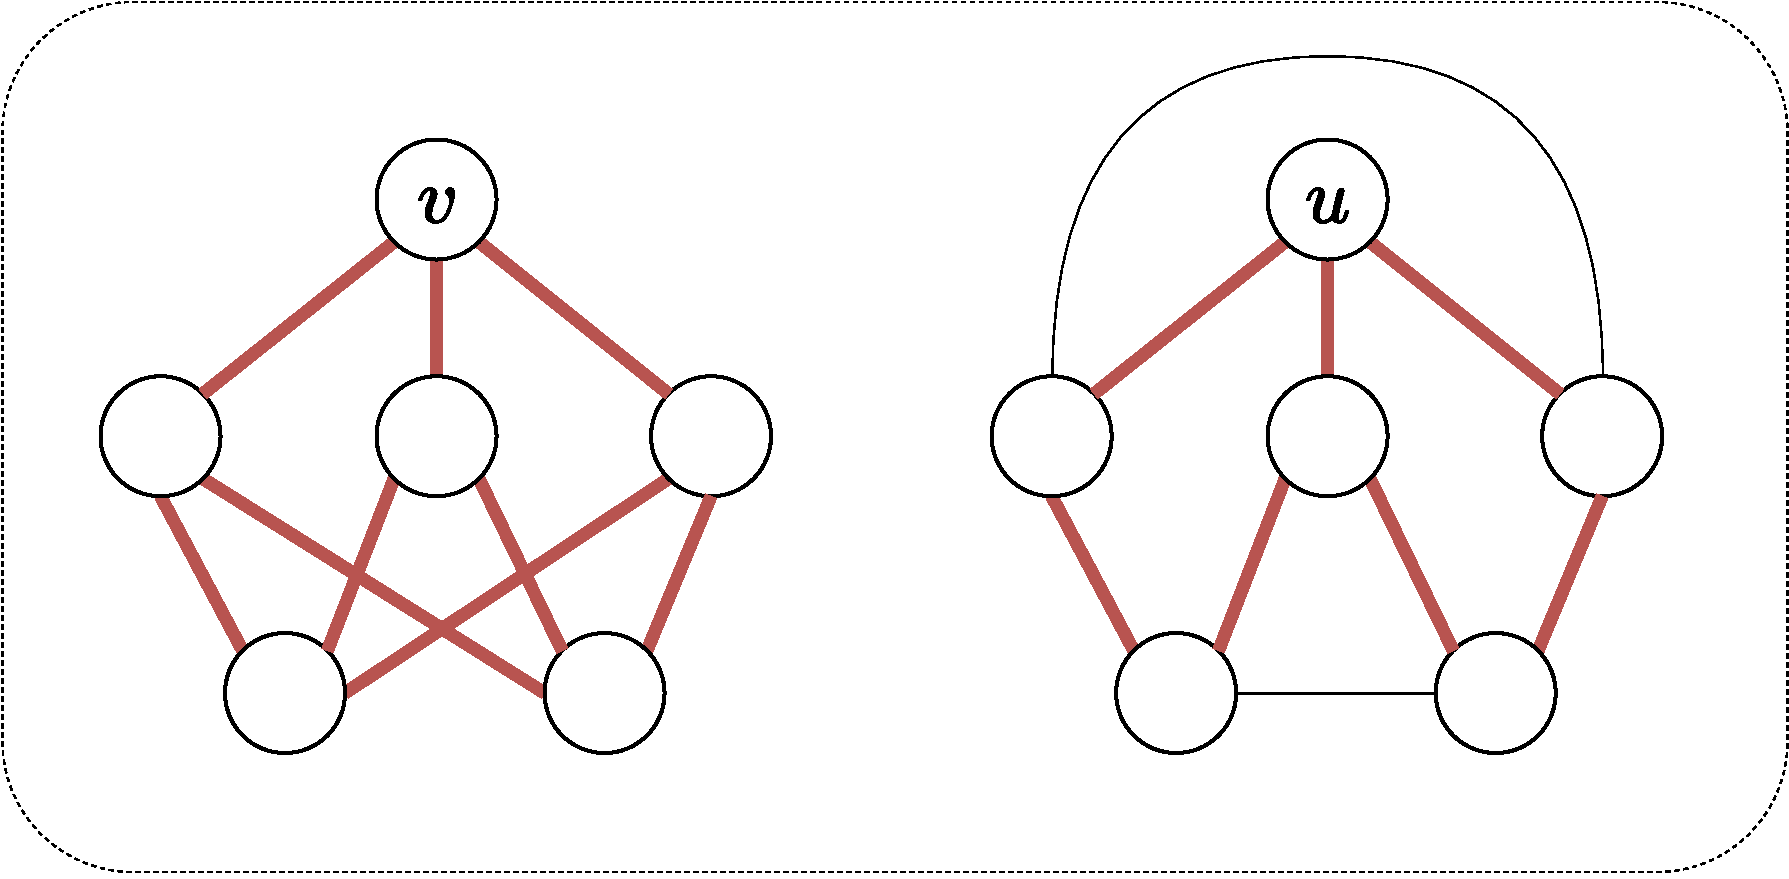
\includegraphics[clip,width=0.8\textwidth]{figures/lemma2_a.pdf}
% \subcaption{Two graphs of non-isomorphic ESPG}
% \label{subfig:espg_non_iso}
% \end{subfigure}%
% \hfill
% \begin{subfigure}{.5\columnwidth}
% \centering
% \captionsetup{width=.9\linewidth}
%         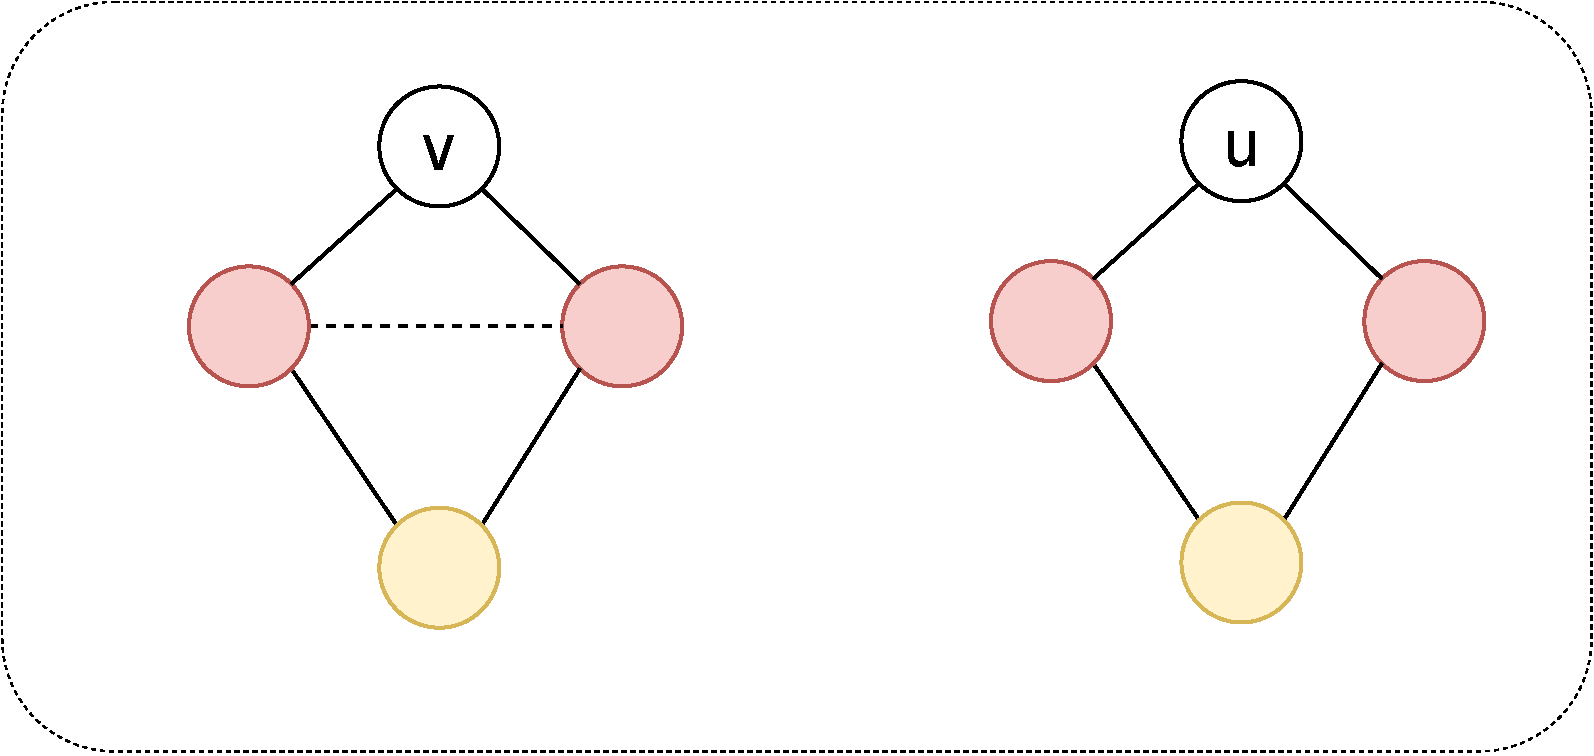
\includegraphics[clip,width=0.8\textwidth]{figures/lemma2_b.pdf}
% \subcaption{Two graphs of isomorphic ESPG}
% \label{subfig:espg_iso}
% \end{subfigure}
% \caption{Couterexamples to prove \cref{lemma:mpnn_esgp}} 
% \label{fig:mpnn_esgp_couterexamples}
% \end{figure*}

\mpnnesgp*
\begin{proof}
Consider vertices $v$ and $u$ and their 1-hop neighbour vertex sets $N_1(v)$ and $N_1(u)$, respectively. We use $\lambda_{\text{WL}}(\cdot)$ to denote the colour mapping of 1-WL.
We show an example where $\lambda_{\text{WL}}(v) = \lambda_{\text{WL}}(u)$ but $S_v\not\simeq S_u$. In \cref{fig:esgp_examples}, $S_v$ and $S_u$ are non-isomorphic; however, we can see $\lambda_{\text{WL}}(v)=\lambda_{\text{WL}}(u)$ because each vertex is adjacent to the same number of vertices. We know from \citet{xu2018powerful} that MPNN's expressivity is upper-bounded by 1-WL; thus, the proof is done.
% We use two counterexamples to prove this lemma. Firstly, we show an example where $\lambda_{\text{WL}}(v) = \lambda_{\text{WL}}(u)$ but $S_v\not\simeq S_u$. In \cref{subfig:espg_non_iso}, $S_v$ and $S_u$ are non-isomorphic; however, we can see $\lambda_{\text{WL}}(v)=\lambda_{\text{WL}}(u)$ because each vertex is adjacent to the same number of vertices. Next, we show an example in \cref{subfig:espg_iso} where $S_v\simeq S_u$ but $h_v \neq h_u$. In this example, although two graphs have isomorphic ESPGs, there is an extra edge (dashed line) between two pink vertices in the left graph, therefore $\lambda_{\text{WL}}(v) \neq \lambda_{\text{WL}}(u)$. We know from \citet{xu2018powerful} that MPNN's expressivity is upper-bounded by 1-WL; thus, MPNN cannot distinguish isomorphic ESPGs.
\end{proof}

% We introduce \cref{corollary:lvc_bfs_path_distance} that is useful for later proofs.
% \begin{restatable}[]{corollary}{lvcbfspathlength}
% \label{corollary:lvc_bfs_path_distance}
% BFC implicitly encodes search path length, i.e. For any two vertices $v \in V_G$ and $u \in V_H$, $\lambda_G(v) = \lambda_H(u)$ only if for each $v'\in N_{\delta}(v)$ there is a $u'\in N_{\delta}(u)$ such that $|P_{v'v}| = |P_{u'v}|$, and vice versa.
% \end{restatable}

% \begin{proof}
% For $\lambda_G(v)=\lambda_H(u)$ to hold, according to \cref{eqn:lvc,eqn:lvc-all}, for each $v' \in N_{\delta}(v)$ there must be a $u' \in N_{\delta}(u)$ such that $\lambda_{v'}(v) = \lambda_{u'}(u)$. So we can assume for $v'$ $|P_{vv'}| \neq |P_{uu'}|$ for all $u' \in N_{\delta}(u)$, and show $\lambda_G(v)=\lambda_H(u)$ cannot hold.
% We prove this by showing if $|P_{vv'}| \neq |P_{uu'}|$ then $\lambda_{v'}(v) \neq \lambda_{u'}(u)$.
% We first show $\lambda_{v'}(v) \neq \lambda_{u'}(u)$ when $|P_{v'v}| < |P_{u'u}|$. We prove this by contradiction.
% Without loss of generality, assuming $P_{v'v}$ is a $\delta$-length path with ordered vertices $(v', w_1, ..., w_{\delta-2}, v)$, we can expand $\lambda_{u'}(u)$ as 
% \begin{align*}
% \lambda_{v'}(v) & := \rho(\lambda(v), \{\!\!\{ \lambda_{v'}(w_{\delta-2}) \}\!\!\}) \\
% \lambda_{v'}(w_{\delta-2}) & := \rho(\lambda(w_{\delta-2}), \{\!\!\{ \lambda_{v'}(w_{\delta-3}) \}\!\!\})  \\
% & ... \\
% \lambda_{v'}(w_{1}) & := \rho(\lambda(w_{1}), \{\!\!\{ \lambda_{v'}(v') \}\!\!\})  \\
% \end{align*}
% Assuming $P_{u'u}$ is a ($\delta+d$)-length path with ordered vertices $(u', w_1', ..., w_d',..., w_{\delta+d-1}', u)$ where $d\in\mathcal{Z}$ and $d \geq 1$, we can expand $\lambda_{u'}(u)$ as
% \begin{align*}
% \lambda_{u'}(u) & := \rho(\lambda(u), \{\!\!\{ \lambda_{u'}(w_{\delta + d -2}') \}\!\!\}) \\
% \lambda_{u'}(w_{\delta+d-2}') & := \rho(\lambda(w_{\delta-2}'), \{\!\!\{ \lambda_{u'}(w_{\delta + d -3}') \}\!\!\})  \\
% & ... \\
% \lambda_{u'}(w_{d}') & := \rho(\lambda(w_{d}'), \{\!\!\{ \lambda_{u'}(w_{d-1}')) \}\!\!\})  \\
% & ... \\
% \lambda_{u'}(w_{1}') & := \rho(\lambda(w_{1}'), \{\!\!\{ \lambda_{u'}({u'}) \}\!\!\})  \\
% \end{align*}
% In order for $\lambda_{v'}(v) = \lambda_{u'}(u)$ to hold, we need
% \begin{equation*}
% \rho(\lambda(v), \{\!\!\{ \lambda_{v'}(w_{\delta-2}) \}\!\!\}) = \rho(\lambda(u), \{\!\!\{ \lambda_{u'}(w_{\delta+d-2}') \}\!\!\})
% \end{equation*}
% Based on injectivity of $\rho(\cdot)$, we must have $\lambda_{v'}(w_{\delta-2}) = \lambda_{u'}(w_{\delta+d-2}')$, which further leads to $\lambda_{v'}(w_{\delta-3}) = \lambda_{u'}(w_{\delta+d-3}')$. Continue doing this until it leads to $\lambda_{v'}(v) = \lambda_{u'}(w_d')$ which can be further expanded as
% \begin{equation*}
% \rho(\lambda(v')) = \rho(\lambda(w_d'), \{\!\!\{ \lambda_{u'}(w_{d-1}') \}\!\!\})
% \end{equation*}
% which obviously breaks injectivity of $\rho(\cdot)$ so must not hold, therefore $\lambda_{v'}(v) \neq \lambda_{u'}(u)$ when $|P_{v'v}| < |P_{u'u}|$. Similarly, we can show $\lambda_{v'}(v) \neq \lambda_{u'}(u)$ when $|P_{v'v}| > |P_{uu'}|$. Hence the proof is done.
% \end{proof}

\dfcinvariance*

\begin{proof}
By showing that $\eta_{\text{dfc}}$ is invariant to vertex search orders, we can prove that $\eta_{\text{dfc}}$ is permutation invariant.

Note that for DFS rooted at vertex $v$, there are multiple search trees if and only if there exist back edges. For a DFS tree $T_v$, any alternative DFS tree can be formed by changing a tree edge to a back edge and swap their directions. If there are no back edges in a DFS tree, the DFS tree is canonical such that the output of $\eta_{\text{dfc}}$ does not change. So below we only consider the case where back edges exist. 

For a non-root vertex $u$ in $G$, there must be one and only one tree edge leading to $u$, i.e. exact one vertex in $\{o:(o,u)\in E_{\text{tree}}^{T_v} \}$. If $Q_u^{T_v}$ in \cref{eqn:dfc_qu} is empty, $u$ is not covered by a back edge and $u$ is not in any cycle because a cycle is formed by at least one back edge~\citep{Cormen_algointro}. Since $u$ is not in any cycle, the vertex $w$ precedes $u$ in $T_v$ is deterministic.

Now we consider the case where $Q_u^{T_v}$ is not empty, which has two further cases. Let $w$ be a vertex preceding $u$ in the tree edge $(w,u)$. 

\begin{itemize}
    \item The first case is when $w$ and $u$ are covered together by a back edge, or by two back edges that crossover each other. In this case, $u$ and $w$ are in the same cycle(s), so $w$ appears in $B_u^{T_v}$. For any alternative search tree to $T_v$, $w$ and $u$ must also be covered together by a back edge, or by two back edges that crossover each other. So the union $\{o: (o,u) \in E_{\text{tree}}^{T_v}   \}
\cup  \{o: o \in B_u^{T_v}\}$ in \cref{eqn:sigma_df} remains the same for all possible search trees. 

\item The second case is when $w$ and $u$ are not covered by a back edge, or are covered by two back edges that do not crossover each other. In this case, $(w,u)$ appears as a tree edge in all possible search trees rooted at $v$, because the tree edge $(w,u)$ is not in any cycles. In this case, $D^{T_v}_u$ remains the same for all search trees, which makes the union $\{o: (o,u) \in E_{\text{tree}}^{T_v}  \}
\cup  \{o: o \in B_u^{T_v}\}$ invariant to traversal order. 
\end{itemize}
Thus, $\eta_{\text{dfc}}$ is invariant to vertex traversal order. The proof is done.
\end{proof}

In the following, we introduce a lemma that is useful for proving \cref{lemma:dfcbiconnectivity}.

\begin{lemma}
\label{lemma:binnect_back_edge_cover}
Each vertex in a biconnected component is covered by at least one DFS back edge.
\end{lemma}
\begin{proof}
A biconnected component is an induced subgraph of $G$ which stays connected by removing any one vertex. Therefore, each vertex in a biconnected component should participate in at least one cycle.
We know a vertex forms a cycle if and only if it is covered by a DFS back edge. Hence, vertices in a biconnected component is covered by at least one DFS back edge.
\end{proof}

\dfcbiconnectivity*
\begin{proof}
We prove the statements in \cref{lemma:dfcbiconnectivity} one by one.
\begin{itemize}
    \item By the definition that a vertex $u$ is a cut vertex of $G$ if removing $u$ increases the number of connected components, \citet{Hopcroft1973-lu} shows that $u$ is a cut vertex if one of the following two conditions is true:
        \begin{enumerate}
            \item $u$ is not the root of a DFS tree, and it has a child $c$ such that no vertex in the subtree rooted with $c$ has a back edge to one of the ancestors in the DFS tree of $u$.
            \item $u$ is the root of a DFS tree, and it has at least two children.
        \end{enumerate}
    \cref{eqn:lvc-all} only computes vertex colour based on search trees where $u$ is not the root, so we can just focus on condition 1. There are two types of cut vertex: one that does not form biconnected components, called the \emph{type-1 cut vertex} (e.g. $v_4$ and $v_5$ in \cref{subfig:dfc2}), and the other that forms biconnected components, called the \emph{type-2 cut vertex} ($v_2$ and $v_6$ in \cref{subfig:dfc2}). We first show that the first statement holds for the type-1 cut vertex.
    
    For a type-1 cut vertex $u$, it is easy to see that we have $D^{T_v}_u = \varnothing$ because of \cref{lemma:binnect_back_edge_cover}. Hence, $\eta_{\text{dfc}}(u,E_{\text{tree}}^{T_v},E_{\text{back}}^{T_v})$ returns a single vertex set containing $w$, where $w$ is the vertex preceding $u$ in the tree edge $(w,u)$. Note that both a type-1 cut vertex and a leaf vertex (a vertex without children) obtain a single vertex set from \cref{eqn:sigma_df}; however, according to Condition 1, a leaf vertex is not a vertex tree. We show that if $u$ is a cut vertex and $x$ is a leaf vertex, $\lambda_G(u)\neq \lambda_G(x)$. We show this by contradiction. A leaf vertex has a degree of 1 while a cut vertex must have a degree larger than 1 (because it connects at least two biconnected components). For $\lambda_G(u) = \lambda_G(x)$ to hold, according to \cref{eqn:lvc-all}, there must be the same number of vertices in $N_{\delta}(u)$ and $N_{\delta}(x)$. 
    Because $x$ is a leaf vertex, there is only one vertex, $w_1$, that contributes to the colour of $u$ without involving other vertices.
    Because $u$ is a cut vertex, there are at least two vertices, $w'_1$ and $w'_2$, that are adjacent to $u$.
    Assuming $\lambda_{w_1}(x) = \lambda_{w'_1}(u)$, there must exist another vertex $ w_2 \in N_{\delta}(x)$ such that $\lambda_{w_2}(x) = \lambda_{w'_2}(u)$ and $w_2$ does not have an edge with $x$. For simplicity, we omit the superscript in \cref{eqn:lvc}, and unpack $\lambda_{w_2}(x)$ and $\lambda_{w'_2}(u)$. We then have 
    $\lambda_{w_2}(x) = \phi \big(  \lambda(x), \psi\left( \{\!\!\{\lambda_{w_2}(w_1)\}\!\!\} \right) \big)$
    and $\lambda_{w'_2}(u) = \phi\big( \lambda(u), \psi\left( \{\!\!\{\lambda_{w'_2}(w'_2)\}\!\!\} \right) \big)$.
    Hence, we need $\lambda_{w_2}(w_1) = \lambda_{w'_2}(w'_2)$.
    Because $\lambda_{w_2}(w_1) = \phi\big(\lambda(w_1),  \psi(\{\!\!\{ \lambda_{w_2}(w_2) \}\!\!\})\big)$,  $\lambda_{w_2}(w_2) = \lambda(w_2)$, and $\lambda_{w_2}(w'_2) = \lambda(w'_2)$, 
    we need to have $\lambda(w'_2) = \phi\big(\lambda(w_1), \psi(\{\!\!\{ \lambda_{w_2}(w_2) \}\!\!\})\big)$ which obviously does not hold. Therefore, if $u$ is a cut vertex and $x$ is a leaf vertex, $\lambda_G(u)\neq \lambda_G(x)$.

    For a type-2 cut vertex $u$, it is obvious that $D^{T_v}_u \neq \varnothing$ and thus the colour of $u$ is clearly different from any leaf vertices or any type-1 cut vertices. So now we just need to show $\lambda_G(u) \neq \lambda_H(x)$ when $x$ is a non-cut vertex in a biconnected component. 
    Because $u$ is a type-2 cut vertex, $\eta_{\text{dfc}}(u,E_{\text{tree}}^{T_v},E_{\text{back}}^{T_v})$ includes all vertices in the biconnected components in which $u$ participates (at least two biconnected components), while for a non-cut vertex $x$, $\eta_{\text{dfc}}(u,E_{\text{tree}}^{T_v},E_{\text{back}}^{T_v})$ includes only vertices in a single biconnected component. %In another word, for a non-cut vertex in a biconnected component, $\eta_{\text{dfc}}(u,E_{\text{tree}}^{T_v},E_{\text{back}}^{T_v})$ contains only vertices in a single biconnected component, while for a type-2 cut vertex, $\eta_{\text{dfc}}(u,E_{\text{tree}}^{T_v},E_{\text{back}}^{T_v})$ contains all vertices in all biconnected components $u$ participates in (at least two biconnected components).
    So a type-2 cut vertex has a different number of vertices in $\eta_{\text{dfc}}(u,E_{\text{tree}}^{T_v},E_{\text{back}}^{T_v})$ comparing with a non-cut vertex.
    Therefore, it is easy to see that $\lambda_G(u) \neq \lambda_H(x)$ when $u$ is a type-2 cut vertex and $x$ is a non-cut vertex in a biconnected component.

    Hence, if $\lambda_G(u)=\lambda_G(x)$, and $x$ is a cut vertex if and only if $u$ is a vertex. The proof for the first statement is done.

    \item According to Tarjan's algorithm for finding cut edges~\citep{Tarjan1974-eb}, in a DFS tree, a tree edge $(u_1, u_2)$ is a cut edge if there is a path from $u_1$ to $u_2$ and every path from $u_1$ to $u_2$ contains edge $(u_1, u_2)$. This can be interpreted as follows: $(u_1, u_2)$ is a cut edge if $u_1$ and $u_2$ are not covered by the same back edge; otherwise, these back edges do not crossover each other. We prove the second statement by contradiction. 
    If $(u_1, u_2)$ is a cut edge and 
    $(x_1, x_2)$ is not a cut edge, assuming 
    $\{\!\!\{ \lambda(u_1), \lambda(u_2)\}\!\!\} = \{\!\!\{ \lambda(x_1), \lambda(x_2)\}\!\!\}$, then $x_1$ and $x_2$ must be covered either by the same back edge or by different back edges that do not crossover each other. Hence, based on \cref{eqn:sigma_df}, $\eta_{\text{dfc}}(x_1,E_{\text{tree}}^{T_v},E_{\text{back}}^{T_v}) = \eta_{\text{dfc}}(x_2,E_{\text{tree}}^{T_v},E_{\text{back}}^{T_v})$. Since $(u_1, u_2)$ is a cut edge, we know $\eta_{\text{dfc}}(u_1,E_{\text{tree}}^{T_v},E_{\text{back}}^{T_v}) \neq \eta_{\text{dfc}}(u_2,E_{\text{tree}}^{T_v},E_{\text{back}}^{T_v})$. This contradicts to $\{\!\!\{ \lambda(u_1), \lambda(u_2)\}\!\!\} = \{\!\!\{ \lambda(x_1), \lambda(x_2)\}\!\!\}$; thus $(x_1, x_2)$ must be a cut edge. We can swap $(x_1, x_2)$ and $(u_1, u_2)$ in the proof to show if $(x_1, x_2)$ is a cut edge, $(u_1, u_2)$ must also be a cut edge. The proof is done for the second statement.

    \item For a graph $G$ to be cut vertex/edge connected, in a DFS tree, there must be a set of back edges that crossover each other and cover all vertices of $G$. Therefore, if $\eta_{\text{dfc}}(u,E_{\text{tree}}^{T_v},E_{\text{back}}^{T_v})$ includes all vertices of $G$, then we have $\eta(u_0,E_{\succ}, E_{\prec}) = \eta(u_1,E_{\succ}, E_{\prec}) = \dots = \eta(u_{N-1},E_{\succ}, E_{\prec})$ for $u_0,u_1,\dots,u_{N-1} \in V_G$. If $H$ is not cut vertex/edge connected, then there must exist at least one vertex $w\in V_H$ such that $w$ is not covered by the same set of crossover back edges that cover other vertices. Thus, 
    $\eta_{\text{dfc}}(w,E_{\text{tree}}^{T_v},E_{\text{back}}^{T_v}) \neq \eta_{\text{dfc}}(x,E_{\text{tree}}^{T_v},E_{\text{back}}^{T_v})$ for $x \in V_H\setminus \{w\}$. We have $\{\!\!\{\lambda(u): u\in V_G\}\!\!\} \neq \{\!\!\{\lambda(u'):u'\in V_H\}\!\!\}$ if $G$ is vertex/edge-biconnected but $H$ is not. The proof is done for the third statement.
    
\end{itemize}
\end{proof}

% We recall \cref{lemma:path_sets}
% \pathsets*
% \begin{proof}
% When $v$ is disconnected, it is easy to see $\mathbb{P}_{v,\delta} = \mathbb{P}_{v,\delta+1}$. When there are no vertices that are $\delta+1$ hops away from $v$, it is also easy to see $\mathbb{P}_{v,\delta} = \mathbb{P}_{v,\delta+1}$. When there is a vertex $u$ that is $\delta+1$ hops away from $v$, there must also be a vertex $w$ that is $\delta$ hops away from $v$ and $w \in \mathcal{P}_{vu}$. According to \cref{def:dit}, we know $\mathcal{P}_{vw} \in \mathbb{P}_{v,\delta}$ and $\mathcal{P}_{vw} \in \mathbb{P}_{v,\delta+1}$ so that $\mathbb{P}_{v,\delta} \subset \mathbb{P}_{v,\delta+1}$. The proof is done.
% \end{proof}

% We recall \cref{lemma:bfsdit}
% \bfsdit*
% \begin{proof}
% Let $\mathcal{P}_{vu}$ be a path found by BFS that starts at $v$ and ends at $u$. If $d(v,u)=1$, it is easy to see $\{v\}\in\{v,u\}$. When $d(v,u)>1$, for any $w \in \mathcal{P}_{vu}$ and $w \neq u$, we have $d(v,w) < d(v,u)$. So $\mathcal{P}_{vw} \subset \mathcal{P}_{vu}$. The proof is done.
% \end{proof}

% We recall \cref{lemma:dfsdit}
% \dfsdit*
% \begin{proof}
% Let $\mathcal{P}_{vu}$ be a path found by DFS that starts at $v$ and ends at $u$. If $d(v,u)=1$, it is easy to see $\{v\}\in\{v,u\}$. When $d(v,u)>1$, 
% before visiting $u$, all vertices $w \in \mathcal{P}_{vu}$ and $u\neq w$ have already been visited because $d(v,w)\leq d(v,u)$. Hence $\mathcal{P}_{vw} \subset \mathcal{P}_{vu}$. The proof is done.
% \end{proof}

\vertexinbiconnectedcomponent*

\begin{proof}

    From the proofs of \cref{lemma:dfcbiconnectivity,lemma:binnect_back_edge_cover}, we know that, if $u$ is in a cycle, $u$ is covered by at least one back edge. So $\eta_{\text{dfc}}(u,E_{\text{tree}}^{T_v},E_{\text{back}}^{T_v})$ contains more than 2 vertices. Since $\lambda(u)=\lambda(u')$, $\eta_{\text{dfc}}(u',E_{\text{tree}}^{T_v},E_{\text{back}}^{T_v})$ also needs to contain more than two vertices, which indicates $u'$ is in a cycle.
    
\end{proof}

\onewlequal*

\begin{proof}
When $\Delta=1$, the vertex colouring function in \cref{eqn:lvc-all} becomes
\begin{equation}
    \lambda^{i+1}(u):= \rho(\lambda^i(u), \{\!\!\{\lambda^{i+1}_v(u)| (u,v)\in E\}\!\!\}).
\end{equation}
Accordingly, we have \cref{eqn:lvc}
\begin{equation}
   \lambda^{i+1}_v(u):= \phi\left(\lambda^i(u), \psi(\{\!\!\{\lambda^{i}(v)\}\!\!\})\right),
\end{equation}
which leads to
\begin{equation}
\label{eqn:lemma_4_6}
    \lambda^{i+1}(u) := \rho\left(\lambda^i(u), \{\!\!\{\phi\left(\lambda^i(u), \psi\left(\{\!\!\{\lambda^{i}(v)\}\!\!\}\right)\right)|(u,v) \in E\}\!\!\}\right).
\end{equation}
Elements in the multiset $\{\!\!\{\phi\left(\lambda^i(u), \psi\left(\{\!\!\{\lambda^{i}(v)\}\!\!\}\right)\right)|(u,v) \in E\}\!\!\}$ only differ in the input of $\psi(\cdot)$. Thus, we can simplify it by defining a new injective function $\kappa(\lambda^i(v)) = \phi\left(\lambda^i(u), \psi\left(\{\!\!\{\lambda^{i}(v)\}\!\!\}\right)\right)$. \cref{eqn:lemma_4_6} becomes 
\begin{equation}
    \lambda^{i+1}(u) := \rho\left(\lambda^i(u), \{\!\!\{\kappa(\lambda^i(v))|(u,v) \in E\}\!\!\}\right),
\end{equation}
which is exactly the vertex colouring function of 1-WL. The proof is done.
\end{proof}


\dfconewl*
\begin{proof}
    Consider two vertices $v$ and $u$, and their 1-hop neighbour vertex sets $N_1(v)$ and $N_1(u)$. We use $\lambda_{\text{dfc}}(\cdot)$ and $\lambda_{\text{wl}}(\cdot)$ to denote the colour refinements by DFC-1 and 1-WL, respectively.
    We first show that if $\lambda_{\text{dfc}}(v) = \lambda_{\text{dfc}}(u)$, then $\lambda_{\text{wl}}(v) = \lambda_{\text{wl}}(u)$. For $\lambda_{\text{dfc}}(v) = \lambda_{\text{dfc}}(u)$ to hold, the number of vertices in $N_1(v)$ must be the same as $N_1(u)$ because of \cref{lemma:equal_neighbour_size}. This means that $v$ and $u$ have the same degree, and thus $\lambda_{\text{wl}}(v) = \lambda_{\text{wl}}(u)$ must hold.
    
    We now show that if $\lambda_{\text{wl}}(v) = \lambda_{\text{wl}}(u)$, $\lambda_{\text{dfc}}(v) = \lambda_{\text{dfc}}(u)$ may not hold. Consider the left graph pair in \cref{fig:circle_examples}, each vertex has a degree of 2 and all vertices have the same colour under 1-WL. However, the number of vertices returned by \cref{eqn:sigma_df} is not the same for the vertices in the left graph and the vertices in the right graph. Specifically, $\eta_{\text{dfc}}(u,E_{\text{tree}}^{T_v},E_{\text{back}}^{T_v})$ returns a set of 3 vertices for each vertex in the left graph and a set of 2 vertices for the right graph. Thus, $\lambda_{\text{dfc}}(v) \neq \lambda_{\text{dfc}}(u)$. This means that DFC-1 can distinguish some pairs of non-isomorphic graphs which 1-WL cannot distinguish. The proof is done.
\end{proof}

\bfcdistinguish*
\begin{proof}
The left graph pair in \cref{fig:circle_examples} can be distinguished by BFC-2 but not by 1-WL. According to \cref{thm:bfcexpressitybeyond}, for any $\delta>2$, BFC-$\delta$ can also distinguish this graph pair. Similarly, the right graph pair in \cref{fig:circle_examples} can be distinguished by BFC-3 but not by 1-WL. So for any $\delta>3$, BFC-$\delta$ can also distinguish this graph pair.
\end{proof}

\dfcdistinguish*
\begin{proof}
The left graph pair in \cref{fig:circle_examples} can be distinguished by DFC-$\delta$ for any $\delta\geq 1$.
The right graph pair in \cref{fig:circle_examples} can be distinguished by DFC-$\delta$ for any $\delta\geq 2$. Both graph pairs cannot be distinguished by 1-WL.
\end{proof}




% \begin{restatable}[]{lemma}{expressityequal_dlvc}
% \label{lemma:expressity_equal}
%  $\text{D-LVC}^{\Delta+1}$ is at least as expressive as $\text{D-LVC}^{\Delta}$ in distinguishing non-isomorphic graphs.
% \end{restatable}

% \begin{proof}
% \label{proof:as_express_as}
% We prove this lemma by contradiction. Assuming there exists two non-isomorphic graphs $G_1$ and $G_2$ which can be distinguished by $\text{D-LVC}^{\Delta}$ but not $\text{D-LVC}^{\Delta+1}$, the colours of any two vertices $u_1$ in $G_1$ and $u_2$ in $G_2$ must be the same by $\text{D-LVC}^{\Delta+1}$ but different by $\text{D-LVC}^{\Delta}$ for any $i$-th iteration where $i=0,1,...,k$. This implies for any $i$-th iteration $\text{D-LVC}^{\Delta+1}$ must have the same multiset of vertex colours for $G_1$ and $G_2$.

% Now it suffices to show that, for any iteration $i$, if the colours of any two vertices in $G_1$ and $G_2$ are the same by $\text{D-LVC}^{\Delta+1}$, then their colours by $\text{D-LVC}^{\Delta}$ must also be the same. we prove this by induction.
% \begin{itemize}
%     \item  for $i=0$, it is obvious to see the initial vertex colours are the same for both $\text{D-LVC}^{\Delta+1}$ and $\text{D-LVC}^{\Delta}$.
%     \item for $i>0$, we assume this statement holds for $i-1$, i.e., $\lambda^{i-1}(u_1) = \lambda^{i-1}(u_2)$, then if the colours of any two vertices in $G_1$ and $G_2$ are the same at the $i$-th iteration by $\text{D-LVC}^{\Delta+1}$, i.e. $\lambda^i_{\Delta+1}(u_1) = \lambda^i_{\Delta+1}(u_2)$, by Eqn.\ref{eqn:lvc-all} we have:
%     \begin{align*}
%         (\lambda^{i-1}(u_1), \{\!\!\{\lambda^{i-1}_{v}(u_1)| v\in N_{\Delta+1}(u_1)\}\!\!\}) \\
%         =  (\lambda^{i-1}(u_2), \{\!\!\{\lambda^{i-1}_{v}(u_2)| v\in N_{\Delta+1}(u_2)\}\!\!\})
%     \end{align*}
%     Since $u_1$ and $u_2$ have the same colour in the $(i-1)$-th iteration, we have
%     \begin{equation}
%         \{\!\!\{\lambda^{i-1}_{v}(u_1)| v\in N_{\Delta+1}(u_1)\}\!\!\}
%         =  \{\!\!\{\lambda^{i-1}_{v}(u_2)| v\in N_{\Delta+1}(u_2)\}\!\!\}
%     \end{equation}
%     In order for the colours of $u_1$ and $u_2$ to be different by $\text{D-LVC}^{\Delta}$, we need 
%     \begin{equation}
%         \{\!\!\{\lambda^{i-1}_{v}(u_1)| v\in N_{\Delta}(u_1)\}\!\!\}
%         \neq  \{\!\!\{\lambda^{i-1}_{v}(u_2)| v\in N_{\Delta}(u_2)\}\!\!\}
%     \end{equation}
%     For simplicity, we define $S_{\Delta}(u) := \{\!\!\{\lambda^{i-1}_{v}(u)| v\in N_{\Delta}(u)\}\!\!\}$. We know $N_{\Delta}(u) \subseteq N_{\Delta+1}(u)$, hence we have
%     \begin{equation}
%         S_{\Delta}(u) \subseteq S_{\Delta+1}(u)
%     \end{equation}
    
%     For the above to hold, we need to have
%     \begin{equation}
%     \label{eqn:contradition_1}
%         (S_{\Delta+1}(u_1) - S_{\Delta}(u_1)) \cap S_{\Delta}(u_2) \neq \emptyset
%     \end{equation}
%     or 
%     \begin{equation}
%     \label{eqn:contradition_2}
%         (S_{\Delta+1}(u_2) - S_{\Delta}(u_2)) \cap S_{\Delta}(u_1) \neq \emptyset
%     \end{equation}
%     From \ref{eqn:lvc-all}, we know
%     \begin{equation}
%         S_{\Delta+1}(u_1) - S_{\Delta}(u_1) =
%         \{\!\!\{\lambda^{i-1}_{v}(u_1)| v\in \left(N_{\Delta+1}(u) - N_{\Delta}(u)\right)\}\!\!\}
%     \end{equation}
    
%     For any vertex $v$ in $N_{\Delta+1}(u) - N_{\Delta}(u)$, there must be at least one vertex $o$ in $N_{\Delta}(u) - N_{\Delta-1}(u)$ so that $(v,o) \in E$.
    
%     That is, $S_{\Delta+1}(u_1) - S_{\Delta}(u_1)$ is the multiset of colours from vertices in $N_{\Delta+1}(u_1) - N_{\Delta}(u_1)$, i.e. vertices that are exactly $\Delta+1$ steps away from $u_1$. $S_{\Delta}(u_2)$ is the multiset of colours from vertices in $N_{\Delta}(u_2)$, i.e. vertices within $\Delta$ steps of $u_2$. From Eqn \ref{eqn:lvc}, we have
%      \begin{equation}
%         \lambda^{i-1}_v(u_1):= \texttt{\rho}(\lambda^{i-1}(u_1), \eta_(v, u_1), \{\!\!\{\lambda^{i-1}_v(w)|(u_1,w)\in E \text{ and }  d(v,u_1) = \Delta\}\!\!\})
%     \end{equation}
%     $\eta_v(v, u_1)$ encodes relative positional information between $v$ and $u_1$ like relative distance, e.g. $\eta(v, u_1) = \Delta+1$ for $S_{\Delta+1}$. In contrary, $S_{\Delta}(u_2)$ only contains positional information up to $\Delta$, e.g. $\eta(v, u_2)=0, \eta(v, u_2)=1, ..., \eta(v, u_2)=\Delta$. And because $\text{rho}(\cdot)$ is injective, we have
%     \begin{equation}
%         (S_{\Delta+1}(u_1) - S_{\Delta}(u_1)) \cap S_{\Delta}(u_2) = \emptyset
%     \end{equation}
%     Similarly, we can show 
%     \begin{equation}
%         (S_{\Delta+1}(u_2) - S_{\Delta}(u_2)) \cap S_{\Delta}(u_1) = \emptyset
%     \end{equation}
%     This contradicts with Eqn \ref{eqn:contradition_1} and Eqn \ref{eqn:contradition_2}. Thus, the following must hold:
%     \begin{equation}
%         \{\!\!\{\lambda^{i-1}_{v}(u_1)| v\in N_{\Delta}(u_1)\}\!\!\}
%         = \{\!\!\{\lambda^{i-1}_{v}(u_2)| v\in N_{\Delta}(u_2)\}\!\!\}
%     \end{equation}
    
%     Hence by Eqn \ref{eqn:lvc-all} and $\lambda^i_{\Delta+1}(u_1) = \lambda^i_{\Delta+1}(u_2)$, we know that the vertex colours of $u_1$ and $u_2$ must be the same by $\text{D-LVC}^{\Delta}$ at the $i$-th iteration.
% \end{itemize}
% This means $\text{D-LVC}^{\Delta}$ cannot distinguish $G_1$ and $G_2$ for any $i$-th iteration where $i=0,1,...,k$, which contradicts the assumption. The proof is done.
% \end{proof}

% We recall \cref{thm:expressitybeyonddlvc}
% \expressitybeyonddlvc*
% The proof is same as \cref{thm:expressity_beyond}


\begin{comment}

\dfcexpressitynotbeyond*
\begin{proof}
    Two examples of graph pairs are shown in \cref{fig:dfc_expressity_delta}, and vertex colours in the left pair are different by DFC-1. Vertex colours in the right pair are different by DFC-2. 
    However, vertex colours in the left pair are the same by DFC-2, and vertex colours in the right pair are the same by DFC-3. That is, when $\delta$ is increased by 1, DFC loses the ability to distinguish the example graph pairs. Therefore increasing $\delta$ may not increase expressivity for DFC, the proof is done.
\end{proof}

\begin{figure*}[ht]
\centering
\begin{subfigure}{.5\textwidth}
\centering
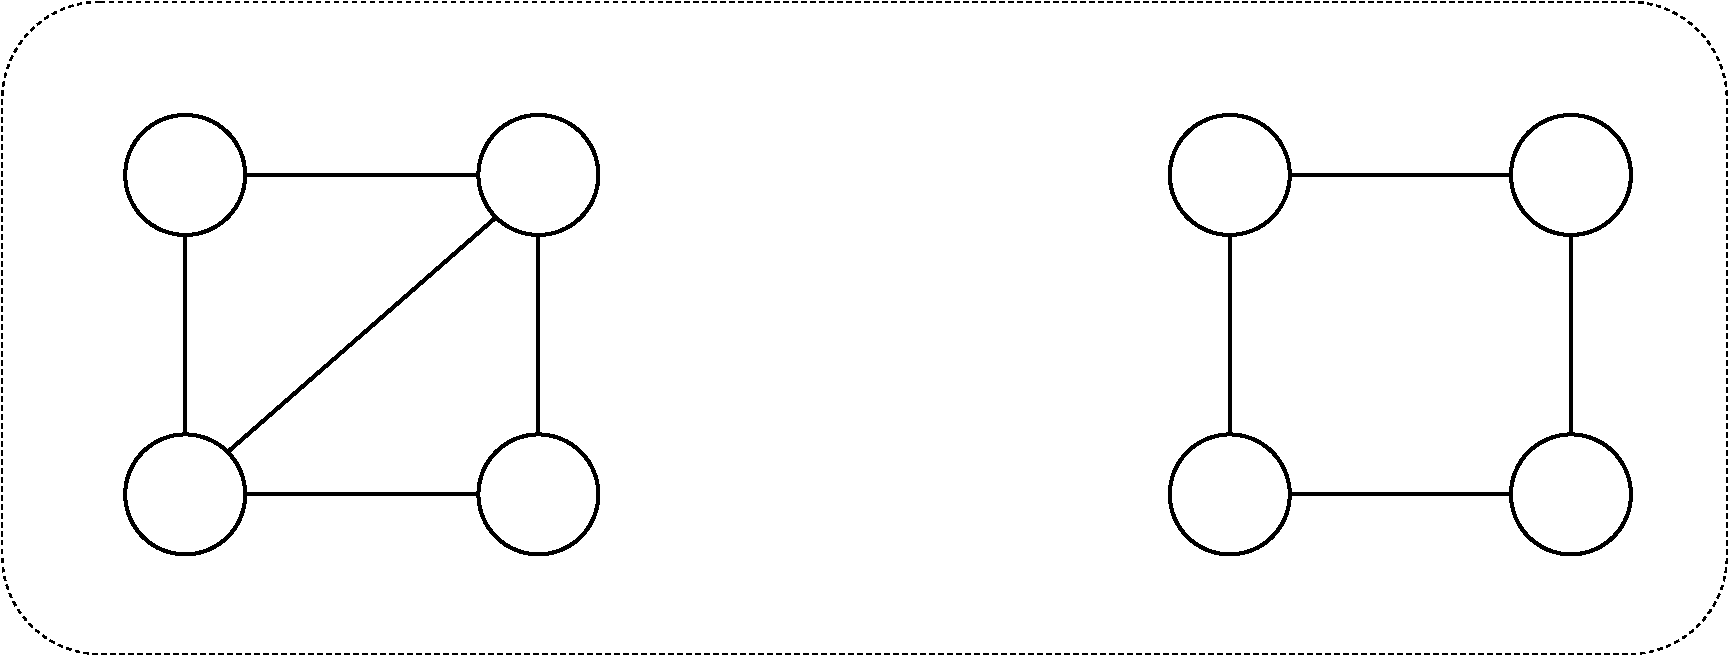
\includegraphics[clip,width=0.7\textwidth]{figures/dfs_expressity_delta_1.pdf}
\end{subfigure}%
\hfill
\begin{subfigure}{.5\textwidth}
\centering
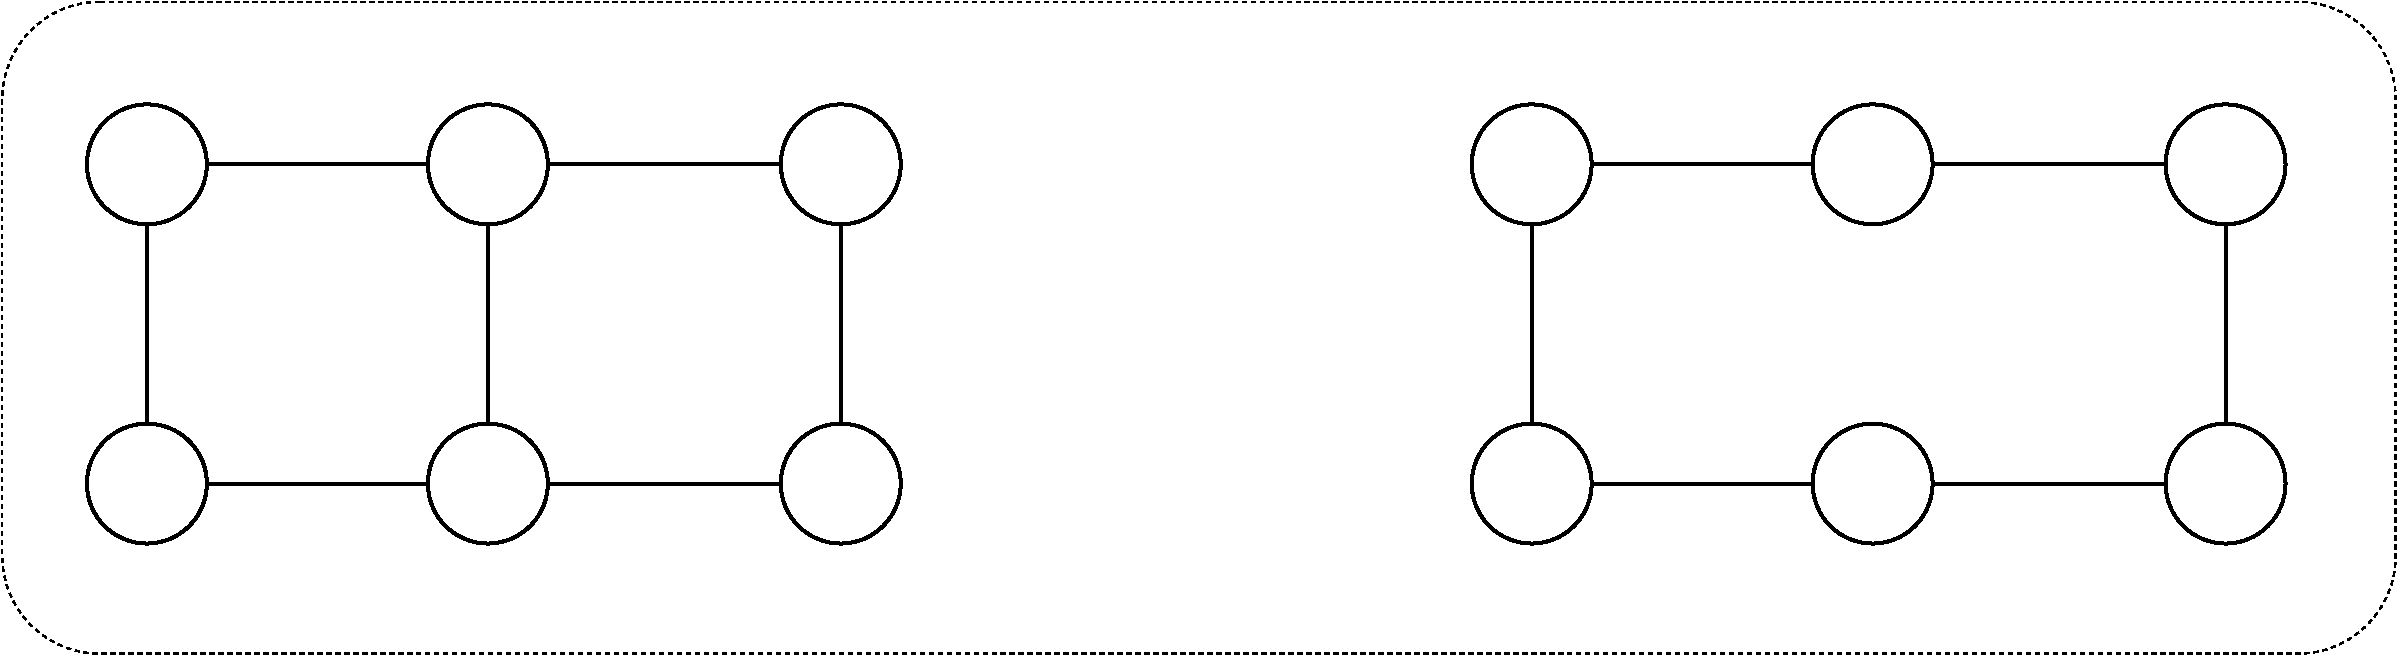
\includegraphics[clip,width=0.95\textwidth]{figures/dfs-expressity_delta_2.pdf}
\end{subfigure}
\caption{Non-isomorphic graph pairs. A pair can be distinguished by DFC-1 but not by DFC-2 (Left). A pair can be distinguished by DFC-2 but not by DFC-3 (Right).} 
\label{fig:dfc_expressity_delta}
\end{figure*}

\end{comment}

Before proving \cref{thm:bfc3wl}, we first define the version of the $k$-WL test studied by~\citet{cai1992optimal}, which is also called \emph{folklore-WL} (FWL)~\cite{morris2019weisfeiler}. Let $\overrightarrow{v}=(v_1, v_2,v_3,\dots, v_k)$ be a $k$-tuple. Then the neighbourhood of $k$-FWL is defined as a set of $n=|V|$ elements:

\begin{equation*}
    \hspace*{-3cm}N^F(\overrightarrow{v}) = \{N^F_w(\overrightarrow{v})|w\in V\},
\end{equation*} 
where each $N^F_w(\overrightarrow{v})$ is defined as:
\begin{equation*}
    \hspace{0.6cm}N^F_w(\overrightarrow{v}) = \{(w, v_2,v_3,\dots, v_k), (v_1,w,v_3,\dots, v_k), \dots, (v_1,v_2,\dots, v_{k-1},w) \}.
\end{equation*}

It is known that $k$-WL is equivalent to ($k$-1)-FWL in distinguishing non-isomorphic graphs when $k >2$~\cite{cai1992optimal}. Thus, below we only need to show that the expressivity of BFC is strictly upper bounded by 2-FWL.

When $k=2$, the neighbourhood of $2$-FWL is a set of $n$ elements of a pair of 2-tuples:

\begin{equation}
    \hspace*{-3cm}N^F(u,v) = \{(u,w),(w,v)|w\in V\}.
\end{equation}

Equivalently, the above equation may be written as:

\begin{equation}\label{equ:2-fwl}
    \hspace*{-3cm}N^F(u,v) = \{(u,w,v)|w\in V\}. 
\end{equation}


Let $G=(V,E)$ be an input graph, $2$-FWL assigns colours to all pairs of vertices of $G$. Initially, there are three colours being assigned: \emph{edge}, \emph{nonedge}, and \emph{self}.
Then the colours of these pairs of vertices are refined iteratively by assigning a new colour to each pair $(u, v)$ depending on the colours of $\{(u,w,v)|w\in V\}$ in $G$. This process continues until the colours of all pairs of vertices stabilize.     

Let $Col(u,v)$ denote the colour of the vertex pair $(u,v)$ by 2-FWL, and $d(u,v)$ denote the shortest-path distance between $u$ and $v$. We have \cref{lemma:bfc2fwl}.

\begin{restatable}[]{lemma}{bfc2fwl}
\label{lemma:bfc2fwl}
Given two pairs of vertices $(u,v)$ and $(u',v')$, if $SPG(u,v)\not\simeq SPG(u',v')$, then $Col(u,v)\neq Col(u',v')$.
\end{restatable}

\begin{proof}
We prove this by induction.

\begin{itemize}
    \item When $d(u,v)=0$ and $d(u',v')=0$, we must have $u=v$ and $u'=v'$. Accordingly, both $SPG(u,v)$ and $SPG(u',v')$ contain only one node. Thus $SPG(u,v)\simeq SPG(u',v')$ and it is impossible to have $SPG(u,v)\not\simeq SPG(u',v')$.

\item When $d(u,v)=1$ and $d(u',v')=1$, we have $(u,v)\in E$ and $(u',v')\in E$. Then both $SPG(u,v)$ and $SPG(u',v')$ contain only one edge. Thus $SPG(u,v)\simeq SPG(u',v')$ and it is impossible to have $SPG(u,v)\not\simeq SPG(u',v')$.


\item When $d(u,v)=2$ and $d(u',v')=2$, we must have $(u,v)\not\in E$ and $(u',v')\not\in E$. By Equation~\ref{equ:2-fwl}, we also know that  
\begin{align*}\label{equ:d2-2-fwl}
      N^F(u,v) = & \{(u,w,v)|(u,w)\in E,(w,v)\in E, w\in V\backslash\{u,v\}\}\cup\\&\{(u,w,v)|(u,w)\in E, (w,v)\not\in E, w\in V\backslash\{u,v\}\}\cup\\   
      &\{(u,w,v)|(u,w)\not\in E, (w,v)\in E, w\in V\backslash\{u,v\}\}\cup\\ 
      &\{(u,w,v)|(u,w)\not\in E, (w,v)\not\in E, w\in V\backslash\{u,v\}\}\cup\\ 
      &\{(u,w,v)|w=u\}\cup\\ 
      &\{(u,w,v)|w=v\} 
\end{align*}
Note that, each of the subsets in the above equation corresponds to a different kind of neighbour in the neighbourhood of $(u,v)$. In this case, equivalently, $SPG(u,v)=(V_{uv}, E_{uv})$ can also be expressed as the subsets of $N^F(u,v)$ that corresponds to three kinds of neighbours in the neighbourhood of $(u,v)$ (Lines 1, 5, and 6 in the above equation):
\begin{align*}
      V_{uv} = &\{u,v\}\cup\{w|(u,w)\in E,(w,v)\in E, w\in V\backslash\{u,v\}\}\\
      E_{uv} = & \{(u,w),(w,v)|(u,w)\in E,(w,v)\in E, w\in V\backslash\{u,v\}\}
\end{align*}
%\begin{align*}
%      SPG(u,v) = & \{(u,w,v)|(u,w)\in E,(w,v)\in E, w\in V\backslash\{u,v\}\}\cup\\
%     &\{u,v\}
%\end{align*}
We know that the colouring of 2-FWL preserves injectivity. Thus, if $SPG(u,v)\not\simeq SPG(u',v')$, it means that their corresponding subsets in $N^F(u,v)$ and $N^F(u',v')$ are not isomorphic. Then $Col(u,v)\neq Col(u',v')$.

\item Now assume that the statement ``if $SPG(u,v)\not\simeq SPG(u',v')$, then $Col(u,v)\neq Col(u',v')$" holds for any two pairs of vertices $(u,v)$ and $(u',v')$ when $d(u,v)=d(u',v')\leq \Delta$. We want to show that this statement will hold for the case $d(u,v)=d(u',v')= \Delta+1$.

When $d(u,v)=\Delta+1$, we may express $SPG(u,v)$ as a tree rooted at vertex $u$, which has a number of children $\{SPG(u_1,v),\dots, SPG(u_q,v)\}$ where $d(u_i,v)=\Delta$ for $1\leq i\leq q$. Accordingly, we may express $SPG(u',v')$ in a similar way. Thus, if $SPG(u,v)\not\simeq SPG(u',v')$, there are two cases:
\begin{itemize}
    \item[(1)] $\{SPG(u,u),SPG(v,v)\}\not\simeq \{SPG(u',u'),SPG(v',v')\}$ \\By our assumption for the case $d(u,v)=d(u',v')\leq \Delta$, we have $\{Col(u,u),Col(v,v)\}\not\simeq \{Col(u',u'),Col(v',v')\}$. Hence, we know that $Col(u,v)\neq Col(u',v')$.
    \item[(2)] $\{SPG(u,u), SPG(v,v)\}\simeq \{SPG(u',u'),SPG(v',v')\}$\\ Without loss of generality, we assume that $SPG(u,u)\simeq SPG(u',u')$ and $SPG(v,v)\simeq SPG(v',v')$. Then in this case $SPG(u,v)\not\simeq SPG(u',v')$ implies that $\{SPG(u_1,v),\dots, SPG(u_q,v)\}\not\simeq \{SPG(u'_1,v'),\dots, SPG(u'_p,v')\}$ where $(u,u_i)\in E$ and $d(u_i,v)=\Delta$ for $1\leq i\leq q$, and $(u',u'_j)\in E$ and $d(u'_j,v')=\Delta$ for $1\leq j\leq p$. Here, $p=q$ must hold; otherwise we immediately have $Col(u,v)\neq Col(u',v')$. By our assumption for the case $d(u,v)=d(u',v')\leq \Delta$, we have $\{Col(u_1,v),\dots, Col(u_q,v)\}\not\simeq \{Col(u'_1,v'),\dots, Col(u'_p,v')\}$. Thus, $Col(u,v)\neq Col(u',v')$ must hold.
\end{itemize}
\end{itemize}
\end{proof}

\bfcthreewl*
\begin{proof}
We first seek to show 3-WL is at least as powerful as BFC-$\delta$. Let $G=(V_G, E_G)$ and $H=(V_H, E_H)$ be two input graphs, according to \cref{lemma:lvcbfs_esgp}, BFC can distinguish graphs only when they have different ESPGs, e.g. $\{\!\!\{\lambda_{S_v}(v): v\in V_G\}\!\!\} \neq \{\!\!\{\lambda_{S_u}(u): u\in V_H\}\!\!\}$. So we just need to show $\{\!\!\{Col(v,v') | v' \in V_G \}\!\!\} \neq \{\!\!\{Col(u,u') | u' \in V_H \}\!\!\}$ for any $v\in V_G$ and $u\in V_H$ when $S_v \not\simeq S_u$. 
$S_v\not\simeq S_u$ implies $\{\!\!\{SPG(v', v): v'\in V_G\}\!\!\} \not\simeq \{\!\!\{SPG(u', u): u\in V_H\}\!\!\}$. According to \cref{lemma:bfc2fwl}, we must have $\{\!\!\{Col(v,v') | v' \in V_G \}\!\!\} \neq \{\!\!\{Col(u,u') | u' \in V_H \}\!\!\}$. Thus 3-WL can distinguish graphs when they have different ESPGs, so 3-WL is at least as powerful as BFC-$\delta$.

Now we seek to show the strictness of this bound, that is 3-WL is strictly more expressive than BFC. We show this by introducing an example graph pair in \cref{fig:bfc3wl}. In this example 3-WL can distinguish the graphs but BFC cannot because the two graphs have isomorphic ESPGs. Therefore the expressiveness of BFC is strictly upper bounded by 3-WL.

\begin{figure*}[ht]
\centering
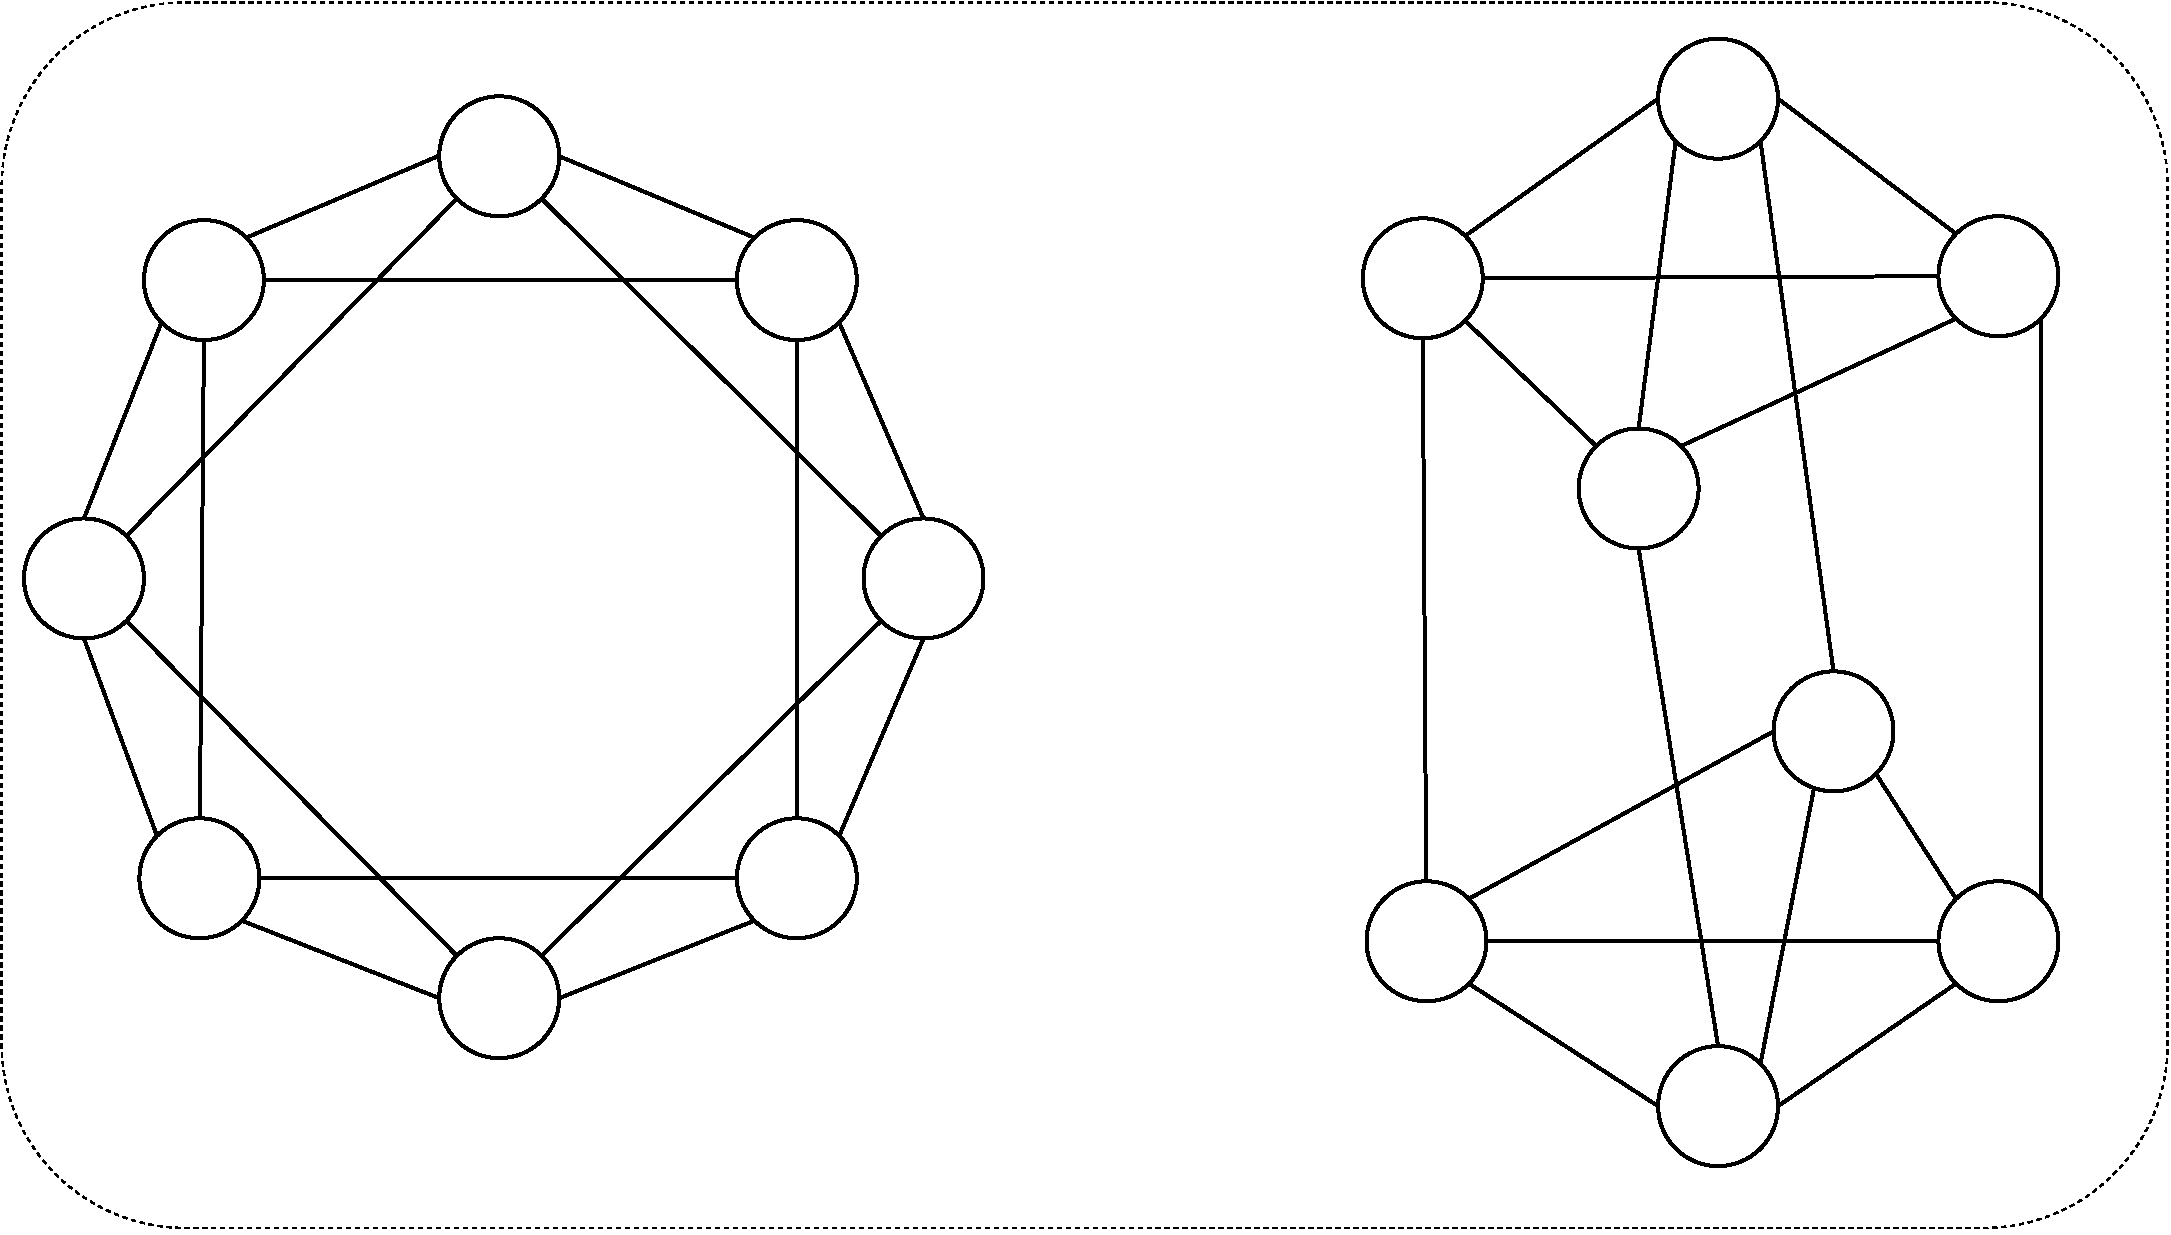
\includegraphics[clip,width=0.4\textwidth]{figures/BFC3WL.pdf}
\caption{A pair of non-isomorphic graphs that can be distinguished by 3-WL but not by BFC.}
\label{fig:bfc3wl}
\end{figure*}

\end{proof}

To prove \cref{thm:bfcexpressitybeyond}, we first introduce \cref{lemma:bfc_equal}.



% \begin{lemma}
% $P_{v}$ and $P_{v'}$ are two simple paths that start at $v$ and $v'$. $u$/$u'$ is a vertex that is $\Delta+1$ hops away from $v$/$v'$, $w$/$w'$ is a vertex that is $\Delta$ hops away from $v$/$v'$. If $\lambda_v(u) = \lambda_v'(u')$ then $\lambda_v(w) = \lambda_v'(w')$.
% \end{lemma}



% \begin{corollary}
% \label{lemma:equal_path_length}
% $P_{vu}$ and $P_{v'u'}$ are two simple path that start at $v$ and $v'$, and ends at $u$ and $u'$ respectively. If $\lambda_v(u) = \lambda_v'(u')$ then $P_{vu}$ and $P_{v'u'}$ have the same number of vertices, i.e. $|P_{vu}| = |P_{v'u'}|$
% \end{corollary}
% \begin{proof}
% We prove this by contradiction. Assuming $|P_{vu}| > |P_{v'u'}|$, we can show it contradicts with $\lambda_v(u) = \lambda_v'(u')$ in a similar as the proof for \cref{lemma:diff_lambda_eqn_path_length}. Similarly, we can show the contradiction when $|P_{vu}| < |P_{v'u'}|$. The proof is done.
% \end{proof}


\begin{restatable}[]{lemma}{expressityequal}
\label{lemma:bfc_equal}
BFC-${\delta+1}$ is at least as expressive as BFC-${\delta}$ in distinguishing non-isomorphic graphs.
\end{restatable}

\begin{proof}
\label{proof:as_express_as}
This lemma requires to show that, for any $i$-th iteration, if BFC-$\delta+1$ must have the same multiset of vertex colours for $G_1$ and $G_2$, then BFC-$\delta$ must also have the same multisets of vertex colours for $G_1$ and $G_2$.
Below we show for any iteration $i$, if the colours of any two vertices in $G_1$ and $G_2$ are the same by BFC-$\delta+1$, then their colours by BFC-$\delta$ must also be the same.
We show this by induction.
 
\begin{itemize}
    \item For $i=0$, it is obvious that the initial vertex colours are the same for BFC-$\delta+1$ and BFC-$\delta$.
    \item For $i>0$, we assume that this statement ``if $\lambda^{i}(u_1) = \lambda^{i}(u_2)$ for BFC-$\delta+1$ then $\lambda^{i}(u_1) = \lambda^{i}(u_2)$ for BFC-$\delta$" holds for the $i$-th iteration, and seek to show that the statement also holds for the $(i+1)$-th iteration. We show this by contradiction. Assuming $\lambda^{i+1}(u_1) = \lambda^{i+1}(u_2)$ hold for BFC-$\delta+1$ but not for BFC-$\delta$, we have
    \begin{equation}
    \label{eqn:expand_delta_plus_1}
        \rho(\lambda^{i}(u_1), \{\!\!\{\lambda^{i}_{v}(u_1)| v\in N_{\delta+1}(u_1)\}\!\!\}) 
        =  \rho(\lambda^{i}(u_2), \{\!\!\{\lambda^{i}_{v}(u_2)| v\in N_{\delta+1}(u_2)\}\!\!\})
    \end{equation}
    and 
    \begin{equation}
    \label{eqn:expand_delta}
        \rho(\lambda^{i}(u_1), \{\!\!\{\lambda^{i}_{v}(u_1)| v\in N_{\delta}(u_1)\}\!\!\}) 
        \neq  \rho(\lambda^{i}(u_2), \{\!\!\{\lambda^{i}_{v}(u_2)| v\in N_{\delta}(u_2)\}\!\!\}).
    \end{equation}
    Because $\lambda^{i+1}(u_1) = \lambda^{i+1}(u_2)$ for BFC-$\delta+1$, we must have $\lambda^{i}(u_1) = \lambda^{i}(u_2)$ for BFC-$\delta+1$. According to our assumption ``if $\lambda^{i}(u_1) = \lambda^{i}(u_2)$ for BFC-$\delta+1$ then $\lambda^{i}(u_1) = \lambda^{i}(u_2)$ for BFC-$\delta$", we have $\lambda^{i}(u_1) = \lambda^{i}(u_2)$ hold for BFC-$\delta$. Thus, we can simplify \cref{eqn:expand_delta_plus_1,eqn:expand_delta} as 
    \begin{equation}
        \label{eqn:color_multiset_delta_plus_1}
        \{\!\!\{\lambda^{i}_{v}(u_1)| v\in N_{\delta+1}(u_1)\}\!\!\}  =  \{\!\!\{\lambda^{i}_{v}(u_2)| v\in N_{\delta+1}(u_2)\}\!\!\}
    \end{equation}
    \begin{equation}
        \label{eqn:color_multiset_delta}
        \{\!\!\{\lambda^{i}_{v}(u_1)| v\in N_{\delta}(u_1)\}\!\!\}  \neq  \{\!\!\{\lambda^{i}_{v}(u_2)| v\in N_{\delta}(u_2)\}\!\!\}
    \end{equation}
    Because $N_{\delta}(u) \subseteq N_{\delta+1}(u)$ and $N_{\delta+1}(u) - N_{\delta}(u) = \{v|d(u,v)=\delta+1\}$, 
    there must exist at least one pair of vertices $u'$ and $u''$, where $d(v,u')=\delta+1$ and $d(v,u'')\leq\delta$, such that $\lambda^{i}_v(u')=\lambda^{i}_v(u'')$.
    This contradicts \cref{lemma:diff_lambda_diff_hop}. So the assumption ``$\lambda^{i+1}(u_1) \neq \lambda^{i+1}(u_2)$ for BFC-$\delta$" must not hold. Thus, the statement ``if $\lambda^{i+1}(u_1) = \lambda^{i+1}(u_2)$ for BFC-$\delta+1$ then $\lambda^{i+1}(u_1) = \lambda^{i+1}(u_2)$ for BFC-$\delta$" holds.
\end{itemize}
This means that, for any iteration $i$, if the colours of any two vertices in $G_1$ and $G_2$ are the same by BFC-$\delta+1$, then their colours by BFC-$\delta$ must also be the same.
The proof is done.
\end{proof}

Now we prove \cref{thm:bfcexpressitybeyond}.
\bfcexpressitybeyond*
\begin{proof}
By \cref{lemma:bfc_equal}, we know that BFC-$\delta+1$ is at least as expressive as BFC-$\delta$. Now we just need to show that there exists at least one pair of non-isomorphic graphs $(\hat{G}_1, \hat{G}_2)$ that can be distinguished by BFC-$\delta+1$ but not by BFC-$\delta$.

Inspired by \citet{wang2023mathscrnwl}, we hereby show a specific construction of such graph pairs using cycles. We construct $\hat{G}_1$ to be two cycles of length $2\delta+1$, and $\hat{G}_2$ to be one cycle of length $4\delta+2$, for any $\delta\geq 1$. $\hat{G}_1$ and $\hat{G}_2$ can be distinguished by BFC-$\delta+1$ but not by BFC-$\delta$. Figure \ref{fig:circle_examples} shows two examples graph pairs constructed using this method. The proof is done.
\end{proof}




%\dfcthreewl*
%\begin{proof}
%    On the one hand, we show DFC-$\delta$ is not always less powerful than 3-WL. DFC-1 can distinguish the strongly regular graph pair shown in \cref{fig:rook_shrikhande} that 3-WL cannot: the Rook's graph of 16 vertices~\citep{Wagon_Weisstein} and the Shrikhande graph~\citep{Shrikhande_graph}. In the Rook graph, each vertex's 1-hop subgraph has a cut vertex, while there is no cut vertex in the Shrikhande graph. So according to \cref{lemma:dfcbiconnectivity}, DFC-1 can distinguish the two graphs. On the other hand, there are also many graphs that 3-WL can distinguish but DFC-1 cannot. For example, the right graph pair in \cref{fig:circle_examples}. Thus DFC-$\delta$ and 3-WL are incomparable.

%\begin{figure*}[ht]
%\centering
%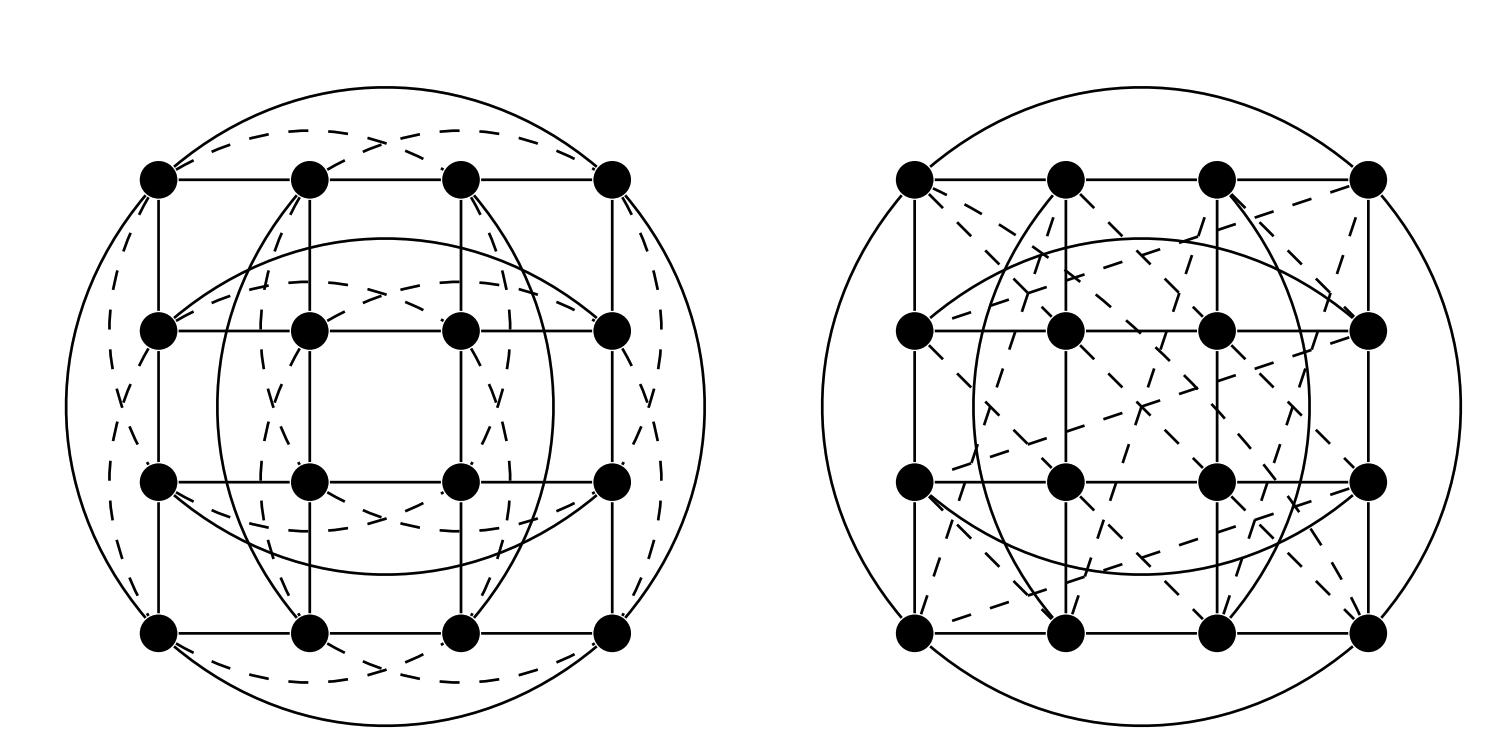
\includegraphics[clip,width=0.4\textwidth]{figures/Shrikhande_Rook_graph.png}
%\caption{The 4x4 rook’s graph G and the Shrikhande graph from \citet{ARVIND202042}. Some edges are dashed for readability.}
%\label{fig:rook_shrikhande}
%\end{figure*}

%\end{proof}

\lvcgnn*

\begin{proof}
    The concatenation operator in Equation \ref{eqn:gnn_layer} preserves injectivity. So Equation \ref{eqn:gnn_layer} is equivalent of replacing $\rho(\cdot)$ in Equation \ref{eqn:lvc-all} with an MLP. The summation operator in Equation \ref{eqn:gnn_huv} is the injective variant of $\psi(\cdot)$ in Equation \ref{eqn:lvc}. The multiplication with $W_c$ is a single-layer MLP that used in place for $\phi(\cdot)$ in Equation \ref{eqn:lvc}. As a universal approximator~\citep{DBLP:journals/nn/Hornik91,DBLP:journals/nn/HornikSW89}, MLP can learn injective functions.
    Hence, \model{} can be shown to be as expressive as LVC following the proof of Theorem 3 by \citet{xu2018powerful}. We leave the details out for brevity.
\end{proof}





